\documentclass[]{book}
\usepackage{lmodern}
\usepackage{amssymb,amsmath}
\usepackage{ifxetex,ifluatex}
\usepackage{fixltx2e} % provides \textsubscript
\ifnum 0\ifxetex 1\fi\ifluatex 1\fi=0 % if pdftex
  \usepackage[T1]{fontenc}
  \usepackage[utf8]{inputenc}
\else % if luatex or xelatex
  \ifxetex
    \usepackage{mathspec}
  \else
    \usepackage{fontspec}
  \fi
  \defaultfontfeatures{Ligatures=TeX,Scale=MatchLowercase}
\fi
% use upquote if available, for straight quotes in verbatim environments
\IfFileExists{upquote.sty}{\usepackage{upquote}}{}
% use microtype if available
\IfFileExists{microtype.sty}{%
\usepackage{microtype}
\UseMicrotypeSet[protrusion]{basicmath} % disable protrusion for tt fonts
}{}
\usepackage[margin=1in]{geometry}
\usepackage{hyperref}
\hypersetup{unicode=true,
            pdftitle={Economics of Superstars},
            pdfauthor={François Geerolf},
            pdfborder={0 0 0},
            breaklinks=true}
\urlstyle{same}  % don't use monospace font for urls
\usepackage{natbib}
\bibliographystyle{apalike}
\usepackage{longtable,booktabs}
\usepackage{graphicx,grffile}
\makeatletter
\def\maxwidth{\ifdim\Gin@nat@width>\linewidth\linewidth\else\Gin@nat@width\fi}
\def\maxheight{\ifdim\Gin@nat@height>\textheight\textheight\else\Gin@nat@height\fi}
\makeatother
% Scale images if necessary, so that they will not overflow the page
% margins by default, and it is still possible to overwrite the defaults
% using explicit options in \includegraphics[width, height, ...]{}
\setkeys{Gin}{width=\maxwidth,height=\maxheight,keepaspectratio}
\IfFileExists{parskip.sty}{%
\usepackage{parskip}
}{% else
\setlength{\parindent}{0pt}
\setlength{\parskip}{6pt plus 2pt minus 1pt}
}
\setlength{\emergencystretch}{3em}  % prevent overfull lines
\providecommand{\tightlist}{%
  \setlength{\itemsep}{0pt}\setlength{\parskip}{0pt}}
\setcounter{secnumdepth}{5}
% Redefines (sub)paragraphs to behave more like sections
\ifx\paragraph\undefined\else
\let\oldparagraph\paragraph
\renewcommand{\paragraph}[1]{\oldparagraph{#1}\mbox{}}
\fi
\ifx\subparagraph\undefined\else
\let\oldsubparagraph\subparagraph
\renewcommand{\subparagraph}[1]{\oldsubparagraph{#1}\mbox{}}
\fi

%%% Use protect on footnotes to avoid problems with footnotes in titles
\let\rmarkdownfootnote\footnote%
\def\footnote{\protect\rmarkdownfootnote}

%%% Change title format to be more compact
\usepackage{titling}

% Create subtitle command for use in maketitle
\newcommand{\subtitle}[1]{
  \posttitle{
    \begin{center}\large#1\end{center}
    }
}

\setlength{\droptitle}{-2em}

  \title{Economics of Superstars}
    \pretitle{\vspace{\droptitle}\centering\huge}
  \posttitle{\par}
  \subtitle{UCLA - Econ 19 - Fall 2018}
  \author{François Geerolf}
    \preauthor{\centering\large\emph}
  \postauthor{\par}
    \date{}
    \predate{}\postdate{}
  
\usepackage{booktabs}
\usepackage{amsthm}
\makeatletter
\def\thm@space@setup{%
  \thm@preskip=8pt plus 2pt minus 4pt
  \thm@postskip=\thm@preskip
}
\makeatother

\usepackage{amsthm}
\newtheorem{theorem}{Theorem}[chapter]
\newtheorem{lemma}{Lemma}[chapter]
\theoremstyle{definition}
\newtheorem{definition}{Definition}[chapter]
\newtheorem{corollary}{Corollary}[chapter]
\newtheorem{proposition}{Proposition}[chapter]
\theoremstyle{definition}
\newtheorem{example}{Example}[chapter]
\theoremstyle{definition}
\newtheorem{exercise}{Exercise}[chapter]
\theoremstyle{remark}
\newtheorem*{remark}{Remark}
\newtheorem*{solution}{Solution}
\begin{document}
\maketitle

{
\setcounter{tocdepth}{2}
\tableofcontents
}
\listoftables
\listoffigures
\chapter*{Econ 19 Material}\label{econ-19-material}
\addcontentsline{toc}{chapter}{Econ 19 Material}

This website contains the class material for \emph{Economics of
Superstars (Econ 19)} I teach at UCLA.

\textbf{All lectures.} Below is an up-to-date version to all lectures
and problem sets in pdf format, as well as a beta ebook version of the
class.

\begin{itemize}
\tightlist
\item
  All lectures. \href{ucla-19-fall2018.pdf}{pdf} /
  \href{ucla-19-fall2018.epub}{epub}
\end{itemize}

\textbf{Lectures.} Below is an html version of all individual lectures,
as well as a timetable of the class.

\begin{itemize}
\tightlist
\item
  Oct 2. \protect\hyperlink{intro-superstars}{Lecture 1} - Introduction
  to the Economics of Superstars
\item
  Oct 16. \protect\hyperlink{statistics-superstars}{Lecture 2} - The
  Statistical Distibution of Superstars: Gaussian VS Pareto
\item
  Oct 30. \protect\hyperlink{music-entertainment-superstars}{Lecture 3}
  - Superstars in Music, Sports and Entertainment
\item
  Nov 13. \protect\hyperlink{presentations1}{Lecture 4} - Presentations
  1
\item
  Nov 27. \protect\hyperlink{presentations2}{Lecture 5} - Presentations
  2
\end{itemize}

\textbf{Presentations.} The presentations will take place during the
last two sessions, on November 13 and November 27. Most of the papers
are \href{https://www.aeaweb.org/issues/313}{taken from a symposium} on
``The Top 1 Percent'' in the \emph{Journal of Economic Perspectives}.
The papers will be presented by groups of 2. Each group should present
for about 15 to 20 minutes. We will then have a 5 to 10 minutes
classroom discussion on the paper. Your presentations should include at
least a summary of the paper, and an overview of the main points. A
critical take, as well as your personal thoughts on the paper, are
strongly encouraged.

\chapter*{Syllabus}\label{syllabus}
\addcontentsline{toc}{chapter}{Syllabus}

\textbf{Lectures:} Tuesdays 2-3:50 pm. Sessions every two weeks,
starting Week 1: Oct 2, Oct 16, Oct 30, Nov 13, Nov 27. Bunche Hall
3170.

\textbf{Course Website:} \url{https://fgeerolf.github.io/econ19/}

\textbf{Moodle Website:}
\url{https://moodle2.sscnet.ucla.edu/course/view/18F-ECON19-1}

\textbf{Course description.} Bradley Cooper, Angelina Jolie, Katy Perry,
Tiger Woods, Tim Cook, Marissa Mayer, and all earned more than 10
million dollars last year according to Forbes. That is more than 300
times the median wage in the United States. Can economics make sense of
these orders of magnitudes? Who among a famous singer, a CEO running an
international organization on several continents, an entrepreneur
creating Microsoft, Apple or Facebook, or a successful Wall Street
trader, creates more ``economic value''? Should inventors, top managers
and CEOs be rewarded more than rock stars or professional athletes? What
are the arguments for and against counteracting the corresponding
increases in inequalities through taxation or other government
interventions? Can we expect the rising ``winner-takes-all'' trend to
continue? The Fiat Lux class \emph{Economics of Superstars} should be a
playful way to first approach basic economic concepts (optimality,
incentives, Pareto distributions, public goods, complementarities,
etc..), and to test the power of economic reasoning as well as its
limits.

\textbf{Grading.} P/NP basis, based on attendance and 30 mn
presentations by groups of 2 or 3, during the last two sessions (Week 7
and Week 9). \emph{To pass this class, you are required to come to all
five classes from beginning to end (per university regulation, because
our classes are 2-hour classes). Please make sure you can make all five
dates before you enroll in this class.}

\textbf{Required readings before classes start.} Sherwin Rosen
(1938-2001), whom the title of this course is borrowed from, wrote about
superstars in The American Scholar in 1983, following his celebrated
\emph{American Economic Review} paper in 1981 (listed under ``To go
further''). You are required to read this piece before classes start:

\begin{itemize}
\tightlist
\item
  \href{https://www.jstor.org/stable/41210977}{Rosen, Sherwin. ``The
  Economics of Superstars.'' The American Scholar 52, no. 4 (1983):
  449--60.}
\end{itemize}

\textbf{Main Readings.} The material for presentations during the last 2
classes can be found in the following eight academic articles. These are
articles from the \emph{Journal of Economic Perspectives}, in
complimentary access from the American Economic Association's website.
They will be assigned on a first come, first served basis. Please
email-me the number of the paper you wish to present, as well as the
name of your partner(s):

\begin{enumerate}
\def\labelenumi{\arabic{enumi}.}
\tightlist
\item
  \href{https://doi.org/10.1257/jep.27.3.3}{Alvaredo, Facundo, Anthony
  B. Atkinson, Thomas Piketty, and Emmanuel Saez. ``The Top 1 Percent in
  International and Historical Perspective.'' Journal of Economic
  Perspectives 27, no. 3 (September 2013): 3--20.}
\item
  \href{https://doi.org/10.1257/jep.27.3.35}{Kaplan, Steven N., and
  Joshua Rauh. ``It's the Market: The Broad-Based Rise in the Return to
  Top Talent.'' Journal of Economic Perspectives 27, no. 3 (September
  2013): 35--56.}
\item
  \href{https://doi.org/10.1257/jep.27.3.57}{Bivens, Josh, and Lawrence
  Mishel. ``The Pay of Corporate Executives and Financial Professionals
  as Evidence of Rents in Top 1 Percent Incomes.'' Journal of Economic
  Perspectives 27, no. 3 (September 2013): 57--78.}
\item
  \href{https://doi.org/10.1257/jep.27.3.21}{Mankiw, N. Gregory.
  ``Defending the One Percent.'' Journal of Economic Perspectives 27,
  no. 3 (September 2013): 21--34.}
\item
  \href{https://doi.org/10.1257/jep.27.3.79}{Corak, Miles. ``Income
  Inequality, Equality of Opportunity, and Intergenerational Mobility.''
  Journal of Economic Perspectives 27, no. 3 (September 2013): 79--102.}
\item
  \href{https://doi.org/10.1257/jep.27.3.103}{Bonica, Adam, Nolan
  McCarty, Keith T. Poole, and Howard Rosenthal. ``Why Hasn't Democracy
  Slowed Rising Inequality?'' Journal of Economic Perspectives 27, no. 3
  (September 2013): 103--24.}
\item
  \href{https://doi.org/10.1257/jep.27.2.73}{Philippon, Thomas, and
  Ariell Reshef. ``An International Look at the Growth of Modern
  Finance.'' Journal of Economic Perspectives 27, no. 2 (May 2013):
  73--96.}
\item
  \href{https://doi.org/10.1257/jep.26.2.119}{Haskel, Jonathan, Robert
  Z. Lawrence, Edward E. Leamer, and Matthew J. Slaughter.
  ``Globalization and U.S. Wages: Modifying Classic Theory to Explain
  Recent Facts.'' Journal of Economic Perspectives 26, no. 2 (May 2012):
  119--40.}
\end{enumerate}

\textbf{Lighter Reading.} The following pieces are written by academic
economists for a broader audience:

\begin{itemize}
\tightlist
\item
  \href{http://www.theguardian.com/business/economics-blog/2012/mar/02/public-salaries-sports-superstars-business}{Kenneth
  Rogoff. ``Public Applauds Huge Salaries for Sports Stars while
  Business Stars Get Abuse.'' \emph{The Guardian}. March 2, 2012.}
\item
  \href{https://www.whitehouse.gov/blog/2013/06/12/rock-and-roll-economics-and-rebuilding-middle-class\#fulltext}{Alan
  B. Krueger. ``Land of Hope and Dreams: Rock and Roll, Economics, and
  Rebuilding the Middle Class. Remarks at the Rock and Roll Hall of
  Fame.'' June 12, 2013.}
\item
  \href{http://www.voxeu.org/article/trade-and-inequality-revisited}{Paul
  Krugman. ``Trade and Inequality, Revisited.'' \emph{Vox EU}. June 15,
  2007.}
\end{itemize}

\textbf{Press articles.} The rise in top incomes is very much in the
news these days. Here is a choice of press articles on the subject:

\begin{itemize}
\tightlist
\item
  \href{http://www.nytimes.com/2010/12/26/business/26excerpt.html?_r=0}{Eduardo
  Porter. ``How Superstars' Pay Stifles Everyone Else.'' \emph{New York
  Times}. December 26, 2010.}
\item
  \href{http://www.newyorker.com/magazine/2014/03/31/forces-of-divergence}{John
  Cassidy. ``Forces of Divergence.'' \emph{New Yorker}. March 31, 2014.}
\item
  \href{http://www.newyorker.com/magazine/2014/11/24/programmers-price}{Lizzie
  Widdicombe. ``The Programmer's Price.'' \emph{New Yorker}. November
  24, 2014.}
\end{itemize}

\textbf{Books (Optional).} To go further, you may want to read the
following related references:

\begin{itemize}
\tightlist
\item
  Piketty, Thomas. Capital in the Twenty-First Century. Harvard
  University Press, 2014.
\item
  Goldin, Claudia, and Lawrence F. Katz. The Race Between Education And
  Technology. Harvard University Press, 2008.
\item
  Moretti, Enrico. The New Geography of Jobs. Houghton Mifflin Harcourt,
  2012.
\item
  Stiglitz, Joseph E. The Price of Inequality: How Today's Divided
  Society Endangers Our Future. W. W. Norton \& Company, 2012.
\end{itemize}

\textbf{To go further (Optional).} My goal will be to try to convey
economic intuitions with the minimum amount of mathematical formalism.
However, you may want to try reading the corresponding academic articles
yourself. They are very often very mathematical, and I certainly do not
expect you to understand their technical derivations. But the
introductions and conclusions usually translate the mathematics into
words, and can actually be fascinating to read. For example, I advise
you to read Sherwin Rosen's introduction to his AER article \emph{The
Economics of Superstars}. (it is the first reference below) You should
also find Handbook chapters and to a lesser extent, the \emph{Annual
Review of Economics}, way more accessible. Again, clicking on the titles
should redirect you directly to a download page. Should the links be
dead, the articles are also available from a computer connected to the
UCLA Wifi, for example through Jstor \url{http://www.jstor.org/} or
directly on Google Scholar \url{https://scholar.google.com/}:

\begin{itemize}
\tightlist
\item
  \href{http://www.jstor.org/stable/1803469}{Rosen, Sherwin. ``The
  Economics of Superstars.'' The American Economic Review 71, no. 5
  (1981): 845--58.}
\item
  \href{https://doi.org/10.2307/2109415}{Hamlen, William A.
  ``Superstardom in Popular Music: Empirical Evidence.'' The Review of
  Economics and Statistics 73, no. 4 (1991): 729--33.}
\item
  \href{https://doi.org/10.1086/425431}{Krueger, Alan B. ``The Economics
  of Real Superstars: The Market for Rock Concerts in the Material
  World.'' Journal of Labor Economics 23, no. 1 (January 1, 2005):
  1--30.}
\item
  \href{https://doi.org/10.1016/S1574-0676(06)01020-9}{Connolly, Marie,
  and Alan B. Krueger. ``Chapter 20 Rockonomics: The Economics of
  Popular Music.'' In Handbook of the Economics of Art and Culture,
  edited by Victor A. Ginsburg and David Throsby, 1:667--719. Elsevier,
  2006.}
\item
  \href{https://doi.org/10.1162/qjec.2009.124.4.1593}{Malmendier,
  Ulrike, and Geoffrey Tate. ``Superstar CEOs.'' The Quarterly Journal
  of Economics 124, no. 4 (November 1, 2009): 1593--1638.}
\end{itemize}

\hypertarget{intro-superstars}{\chapter{Introduction to the Economics of
Superstars}\label{intro-superstars}}

\section{Basic Information}\label{basic-information}

\textbf{Lectures:} Tuesdays 2-3:50 pm. Sessions every two weeks,
starting Week 1: Oct 2, Oct 16, Oct 30, Nov 13, Nov 27. Bunche Hall
3170. \emph{To pass this class, you are required to come to all five
classes from beginning to end (per university regulation, because our
classes are 2-hour classes). Please make sure you can make all five
dates before you enroll in this class.}

\textbf{Course Website:} \url{https://fgeerolf.github.io/econ19/}

\textbf{Moodle Website:}
\url{https://moodle2.sscnet.ucla.edu/course/view/18F-ECON19-1}

\textbf{Course description.} Bradley Cooper, Angelina Jolie, Katy Perry,
Tiger Woods, Tim Cook, Marissa Mayer, and all earned more than 10
million dollars last year according to Forbes. That is more than 300
times the median wage in the United States. Can economics make sense of
these orders of magnitudes? Who among a famous singer, a CEO running an
international organization on several continents, an entrepreneur
creating Microsoft, Apple or Facebook, or a successful Wall Street
trader, creates more ``economic value''? Should inventors, top managers
and CEOs be rewarded more than rock stars or professional athletes? What
are the arguments for and against counteracting the corresponding
increases in inequalities through taxation or other government
interventions? Can we expect the rising ``winner-takes-all'' trend to
continue? The Fiat Lux class \emph{Economics of Superstars} should be a
playful way to first approach basic economic concepts (optimality,
incentives, Pareto distributions, public goods, complementarities,
etc..), and to test the power of economic reasoning as well as its
limits.

\textbf{Grading.} P/NP basis, based on attendance and 30 mn
presentations by groups of 2 or 3, during the last two sessions (Week 7
and Week 9). \emph{To pass this class, you are required to come to all
five classes from beginning to end (per university regulation, because
our classes are 2-hour classes). Please make sure you can make all five
dates before you enroll in this class.}

\textbf{Required readings before classes start.} Sherwin Rosen
(1938-2001), whom the title of this course is borrowed from, wrote about
superstars in The American Scholar in 1983, following his celebrated
\emph{American Economic Review} paper in 1981 (listed under ``To go
further''). You are required to read this piece before classes start:

\begin{itemize}
\tightlist
\item
  \href{https://www.jstor.org/stable/41210977}{Rosen, Sherwin. ``The
  Economics of Superstars.'' The American Scholar 52, no. 4 (1983):
  449--60.}
\end{itemize}

\textbf{Main Readings.} The material for presentations during the last 2
classes can be found in the following eight academic articles. These are
articles from the \emph{Journal of Economic Perspectives}, in
complimentary access from the American Economic Association's website.
They will be assigned on a first come, first served basis. Please
email-me the number of the paper you wish to present, as well as the
name of your partner(s):

\begin{enumerate}
\def\labelenumi{\arabic{enumi}.}
\tightlist
\item
  \href{https://doi.org/10.1257/jep.27.3.3}{Alvaredo, Facundo, Anthony
  B. Atkinson, Thomas Piketty, and Emmanuel Saez. ``The Top 1 Percent in
  International and Historical Perspective.'' Journal of Economic
  Perspectives 27, no. 3 (September 2013): 3--20.}
\item
  \href{https://doi.org/10.1257/jep.27.3.35}{Kaplan, Steven N., and
  Joshua Rauh. ``It's the Market: The Broad-Based Rise in the Return to
  Top Talent.'' Journal of Economic Perspectives 27, no. 3 (September
  2013): 35--56.}
\item
  \href{https://doi.org/10.1257/jep.27.3.57}{Bivens, Josh, and Lawrence
  Mishel. ``The Pay of Corporate Executives and Financial Professionals
  as Evidence of Rents in Top 1 Percent Incomes.'' Journal of Economic
  Perspectives 27, no. 3 (September 2013): 57--78.}
\item
  \href{https://doi.org/10.1257/jep.27.3.21}{Mankiw, N. Gregory.
  ``Defending the One Percent.'' Journal of Economic Perspectives 27,
  no. 3 (September 2013): 21--34.}
\item
  \href{https://doi.org/10.1257/jep.27.3.79}{Corak, Miles. ``Income
  Inequality, Equality of Opportunity, and Intergenerational Mobility.''
  Journal of Economic Perspectives 27, no. 3 (September 2013): 79--102.}
\item
  \href{https://doi.org/10.1257/jep.27.3.103}{Bonica, Adam, Nolan
  McCarty, Keith T. Poole, and Howard Rosenthal. ``Why Hasn't Democracy
  Slowed Rising Inequality?'' Journal of Economic Perspectives 27, no. 3
  (September 2013): 103--24.}
\item
  \href{https://doi.org/10.1257/jep.27.2.73}{Philippon, Thomas, and
  Ariell Reshef. ``An International Look at the Growth of Modern
  Finance.'' Journal of Economic Perspectives 27, no. 2 (May 2013):
  73--96.}
\item
  \href{https://doi.org/10.1257/jep.26.2.119}{Haskel, Jonathan, Robert
  Z. Lawrence, Edward E. Leamer, and Matthew J. Slaughter.
  ``Globalization and U.S. Wages: Modifying Classic Theory to Explain
  Recent Facts.'' Journal of Economic Perspectives 26, no. 2 (May 2012):
  119--40.}
\end{enumerate}

\textbf{Lighter Reading.} The following pieces are written by academic
economists for a broader audience:

\begin{itemize}
\tightlist
\item
  \href{http://www.theguardian.com/business/economics-blog/2012/mar/02/public-salaries-sports-superstars-business}{Kenneth
  Rogoff. ``Public Applauds Huge Salaries for Sports Stars while
  Business Stars Get Abuse.'' \emph{The Guardian}. March 2, 2012.}
\item
  \href{https://www.whitehouse.gov/blog/2013/06/12/rock-and-roll-economics-and-rebuilding-middle-class\#fulltext}{Alan
  B. Krueger. ``Land of Hope and Dreams: Rock and Roll, Economics, and
  Rebuilding the Middle Class. Remarks at the Rock and Roll Hall of
  Fame.'' June 12, 2013.}
\item
  \href{http://www.voxeu.org/article/trade-and-inequality-revisited}{Paul
  Krugman. ``Trade and Inequality, Revisited.'' \emph{Vox EU}. June 15,
  2007.}
\end{itemize}

\textbf{Press articles.} The rise in top incomes is very much in the
news these days. Here is a choice of press articles on the subject:

\begin{itemize}
\tightlist
\item
  \href{http://www.nytimes.com/2010/12/26/business/26excerpt.html?_r=0}{Eduardo
  Porter. ``How Superstars' Pay Stifles Everyone Else.'' \emph{New York
  Times}. December 26, 2010.}
\item
  \href{http://www.newyorker.com/magazine/2014/03/31/forces-of-divergence}{John
  Cassidy. ``Forces of Divergence.'' \emph{New Yorker}. March 31, 2014.}
\item
  \href{http://www.newyorker.com/magazine/2014/11/24/programmers-price}{Lizzie
  Widdicombe. ``The Programmer's Price.'' \emph{New Yorker}. November
  24, 2014.}
\end{itemize}

\textbf{Books (Optional).} To go further, you may want to read the
following related references:

\begin{itemize}
\tightlist
\item
  Piketty, Thomas. Capital in the Twenty-First Century. Harvard
  University Press, 2014.
\item
  Goldin, Claudia, and Lawrence F. Katz. The Race Between Education And
  Technology. Harvard University Press, 2008.
\item
  Moretti, Enrico. The New Geography of Jobs. Houghton Mifflin Harcourt,
  2012.
\item
  Stiglitz, Joseph E. The Price of Inequality: How Today's Divided
  Society Endangers Our Future. W. W. Norton \& Company, 2012.
\end{itemize}

\textbf{To go further (Optional).} My goal will be to try to convey
economic intuitions with the minimum amount of mathematical formalism.
However, you may want to try reading the corresponding academic articles
yourself. They are very often very mathematical, and I certainly do not
expect you to understand their technical derivations. But the
introductions and conclusions usually translate the mathematics into
words, and can actually be fascinating to read. For example, I advise
you to read Sherwin Rosen's introduction to his AER article \emph{The
Economics of Superstars}. (it is the first reference below) You should
also find Handbook chapters and to a lesser extent, the \emph{Annual
Review of Economics}, way more accessible. Again, clicking on the titles
should redirect you directly to a download page. Should the links be
dead, the articles are also available from a computer connected to the
UCLA Wifi, for example through Jstor \url{http://www.jstor.org/} or
directly on Google Scholar \url{https://scholar.google.com/}:

\begin{itemize}
\tightlist
\item
  \href{http://www.jstor.org/stable/1803469}{Rosen, Sherwin. ``The
  Economics of Superstars.'' The American Economic Review 71, no. 5
  (1981): 845--58.}
\item
  \href{https://doi.org/10.2307/2109415}{Hamlen, William A.
  ``Superstardom in Popular Music: Empirical Evidence.'' The Review of
  Economics and Statistics 73, no. 4 (1991): 729--33.}
\item
  \href{https://doi.org/10.1086/425431}{Krueger, Alan B. ``The Economics
  of Real Superstars: The Market for Rock Concerts in the Material
  World.'' Journal of Labor Economics 23, no. 1 (January 1, 2005):
  1--30.}
\item
  \href{https://doi.org/10.1016/S1574-0676(06)01020-9}{Connolly, Marie,
  and Alan B. Krueger. ``Chapter 20 Rockonomics: The Economics of
  Popular Music.'' In Handbook of the Economics of Art and Culture,
  edited by Victor A. Ginsburg and David Throsby, 1:667--719. Elsevier,
  2006.}
\item
  \href{https://doi.org/10.1162/qjec.2009.124.4.1593}{Malmendier,
  Ulrike, and Geoffrey Tate. ``Superstar CEOs.'' The Quarterly Journal
  of Economics 124, no. 4 (November 1, 2009): 1593--1638.}
\end{itemize}

\section{\texorpdfstring{Some defining features of ``Superstar
Economics''}{Some defining features of Superstar Economics}}\label{some-defining-features-of-superstar-economics}

During this first course, we start discussing around Sherwin Rosen's
\emph{Economics of Superstars} article in \emph{The American Scholar}.
\href{https://en.wikipedia.org/wiki/Sherwin_Rosen}{Sherwin Rosen}
(1938-2001) was a great American labor economist, who might have gone on
to win the Nobel Memorial Prize in Economic Sciences. Sherwin Rosen's
general audience article on \emph{The Economics of Superstars} is very
dense and has very much to it, but Sherwin Rosen discusses a number of
strong points which we shall come back to.

He argues that markets where superstars are important are characterized
by a \textbf{number of common features}, which we go through next:

\begin{itemize}
\tightlist
\item
  \protect\hyperlink{superstar-incomes}{Superstars can earn
  extra-ordinary sums.}
\item
  \protect\hyperlink{inequality}{The revenues of superstars are very
  heterogeneous.}
\item
  \protect\hyperlink{scale}{Superstar operate on a scale so large that
  the market is divided over a handful of participants.}
\end{itemize}

To summarise, markets where superstar economics operate are
characterized by large, unequal incomes, which are distributed among a
handful of participants. We develop each one of these arguments next.

\hypertarget{superstar-incomes}{\subsection{Large revenues for
superstars}\label{superstar-incomes}}

Sherwin Rosen's superstar paper was written in 1983, therefore, all the
orders of magnitude that he gives need to be adjusted to be comparable
to today's numbers. There are two main reasons why his 1.2 million
figure for a basketball player on a losing team needs to be adjusted.
First, there has been considerable price inflation in the United States
since 1983, so that 1.2 million in 1983 could buy much more then than it
can buy now. Second, there has been quite a lot of per capita GDP growth
as well, so that on average people were much poorer in 1983, which makes
the 1.2 million figure even more impressive.

Using the time series of GDP per capita in current U.S. dollars allows
to account for both problems at the same time. One may find one such
series at the following link:
\url{https://db.nomics.world/WB/WDI/NY.GDP.PCAP.CD-US}. The data which
is then obtained is plotted below. I also give the values for GDP per
capita (as well as, for your information, the values for Real GDP per
capita, in 2010 dollars).

A simple proportional rule allows us to conclude that in order to
convert 1983 dollars to 2017 dollars, taking into account inflation as
well as per capita GDP growth, we need to multiply by a factor of
59531.66/15561.43 = 3.83. Table \ref{tab:real-gdp-per-capita} shows the
numbers used to make that calculation.



\begin{figure}

{\centering 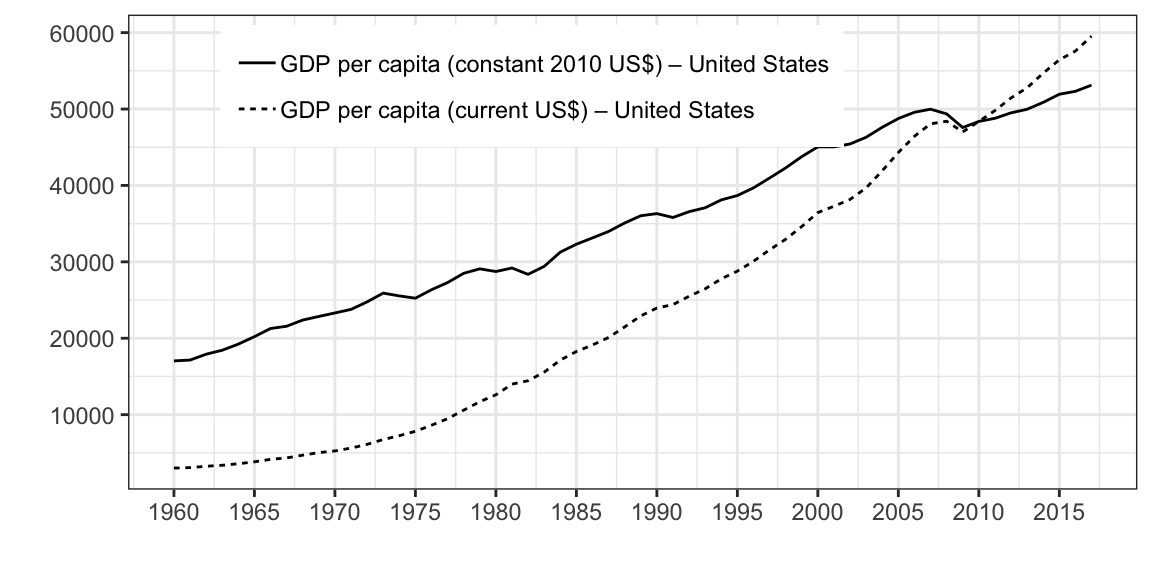
\includegraphics[width=1\linewidth]{ucla-19-fall2018_files/figure-latex/fig-gdp-per-capita-1} 

}

\caption{\textsc{Real GDP Per Capita.}}\label{fig:fig-gdp-per-capita}
\end{figure}



\label{tab:real-gdp-per-capita}\textsc{Real GDP Per Capita.}

year

GDP per capita

Real GDP per capita

1983

15,561

29,406

1990

23,954

36,312

2000

36,450

45,056

2010

48,375

48,375

2017

59,532

53,129

This allows to convert Sherwin Rosen's examples as follows.



\label{tab:rosen-examples}\textsc{Sherwin Rosen (1981)'s examples.}

Star

1983 Income

2017 Income

Basketball player on a losing team

800,000

3,060,472

Television interviewer

2,000,000

7,651,181

Typical NBA Player

250,000

956,398

Boxer of championship caliber (Sugar Ray Loonard)

30,000,000

114,767,717

\hypertarget{inequality}{\subsection{Heterogeneous revenues for
superstars}\label{inequality}}

\hypertarget{scale}{\subsection{Large scale for
superstars}\label{scale}}

The ``scale'' that superstars are able to reach is so potentially large
that the whole market size is in fact divided over a only a handful of
participants in all activities that superstars are engaged in:

\begin{quote}
The first thing to be said in this connection is that certain economic
activities admit extreme concentration of both personal reward and
market size among a handful of participants. Every economic activity
supports considerable diversity of talent and significant inequality in
the personal distribution of rewards. Activities where superstars are
found differ from those in which most of us make our livings by
supporting much less diversity and much more inequality, in the
distribution of earnings. The bulk of earnings goes to relatively small
numbers of practitioners-typically, the few regarded as among the best
in their fields.
\end{quote}

Sherwin Rosen also notes that industrial firms are typically not allowed
to operate at such large scales - because of worries that this would
prevent needed competition. Indeed, there are laws against antitrust,
which are supposed to constrain firms in their ability to raises prices,
which might be detrimental for consumers. However, no such restrictions
exist for individuals, who however are often disproportionately
dominating the market that they operate in (at a moment in time, there
are only a handful of singers who are able to fill in a large stadium):

\begin{quote}
Similar distributions of earnings in the industrial sector would
ultimately come to the attention of the Federal Trade Commission or the
Justice Department, but so far as I know, proceedings in restraint of
trade were never brought against Caruso, Babe Ruth, Picasso, or the
Beatles.
\end{quote}

Because of such scales, many would-be superstars actually never make it
to the top. For example, in boxing, while Sugar Ray leonard has retired
after a relatively brief carrer with wealth on the order of \$30
million, others struggle:

\begin{quote}
The median boxer cannot even make a living at the game an difficulty
generating more than a few thousand per year. Only hopefuls, including
both those with genuine prospects and those have not yet perceived how
dim their prospects really are, can sustain interest and commitment in
boxing at those earnings.
\end{quote}

These superstar phenomena imply that:

\begin{quote}
The National Basketball Association has about 250 players; there is
probably a lesser number of tournament- quality golfers and tennis
players; and there are at most a few dozen highly successful boxers. The
number of people attempting to break into the top echelons is larger by
many orders of magnitude.
\end{quote}

\subsection{The reward structure is highly nonlinear in measurable
talent and
ability}\label{the-reward-structure-is-highly-nonlinear-in-measurable-talent-and-ability}

Sherwin Rosen notes that where superstars are found, the scale of
rewards appears to rise more than proportionately with talent and
ability.

\begin{quote}
These examples point to another characteristic of the activities where
superstars are found. Rewards and the probability of success appear to
rise more than proportionately with talent and ability. In this we are
on a little dangerous ground because in many instances it is difficult
to find objective measures of personal productivity.
\end{quote}

Here, Sherwin Rosen is trying to get at an objective measure of
different abilities. He notes that abilities are actually not that
different, and that a small different can matter a ton. He takes two
examples. First, football:

\begin{quote}
If in football a running back is half a step quicker than the defense,
that might have enormous effect on his productivity.
\end{quote}

Second, golf:

\begin{quote}
The top five money winners on the pro golf tour have annual stroke
averages that are less than 5 percent lower than the fiftieth or
sixtieth ranking players, yet they earn four or five times as much
money.
\end{quote}

Finally, baseball:

\begin{quote}
A twenty-game winning pitcher in baseball earns far more than the sum of
two ten-game winners.
\end{quote}

This is true in music, as well:

\begin{quote}
Interestingly, income differences between first-rank and second-rank
performers are substantial, even though, in a blind hearing, an
infinitesimal portion of the audience could detect more than minor
differences among them.
\end{quote}

\subsection{Use of audiences / Media
audiences}\label{use-of-audiences-media-audiences}

Media attention is paramount:

\begin{quote}
For the phenomenon of superstar income to exist, certain conditions must
exist alongside it. The attention of the media to t he activities in
which the superstars engage is one such condition. This becomes evident
in the world of show business, of which professional sports might be
considered a subset; but it is also evident in arts and letters, two
other fields that produce superstars. Show business first. Plausibly
informed opinion has it that the number of full-time comedians in the
United States does not exceed a few hundred. This is probably a smaller
number than was employed in the days of vaudeville. Among contemporary
comedians, the most popular are reported to earn extraordinary sums-an d
none earn more than those who appear regularly on television. Again, the
capacity of television to produce large incomes is manifest in the
enormous salaries paid to news broadcasters, especially those who work
for t he networks and for stations located in large local markets such
as New York and Chicago.
\end{quote}

\begin{quote}
The other element has to do with certain peculiarities in the technology
of the production of services through the use of audiences. These
activities must admit duplication of a kind so that a person - the
superstar - can deliver services to many buyers simultaneously. Once
again, here the use of media is instrumental.
\end{quote}

\subsection{Poor talent is an inedequate substitute for superior
talent}\label{poor-talent-is-an-inedequate-substitute-for-superior-talent}

\begin{quote}
Wherever superstars are to be found, I believe at least one of two
elements will also be found-elements that are necessary to support and
sustain both stars and superstars. One element is that the technology of
consumption or use of the services provided by the activity must be such
that poor talent is an inadequate substitute for superior talent
\end{quote}

\begin{quote}
Sometimes these differences are inherent in the valuations put upon
services by buyers. If one surgeon is 10 percent more successful in
saving lives than another, who among us would not be willing to pay much
more than a 10 percent premium to have the more skillful person perform
the operation? A company engaged in a \$30 million treble-damages
lawsuit is rash to scrimp on the legal talent it engages. Stockholders
and directors would look askance at ring mediocre talents under those
circumstances.
\end{quote}

In the case of the music industry:

\begin{quote}
Hearing a succession of second- rate singers does not measure up to
hearing one outstanding performance by Placido Domingo. Contracting for
a legal defense with two lawyers, each of whom would be likely to lose
the case half the time, would not elevate the probability of winning
much above one-half and may actually decrease it.
\end{quote}

\subsection{Limited costs of
duplication}\label{limited-costs-of-duplication}

\begin{quote}
The superstar is someone whose audience is enormous relative to the
scale on which most of us operate. Personal markets of that magnitude
are almost exclusively sustained by use of media as a cooperating
resource. These markets represent technologies that, in effect, allow a
person to clone himself at little cost. More precisely, costs do not
increase nearly in proportion to market size; and if costs are the same,
the more tickets that can be sold is, as they say, all gravy. Once an
author delivers a manuscript to a publisher, it can be duplicated at
small expense practically indefinitely. A television or radio program is
communicated virtually costlessly and identically to whomever happens to
tune in. The performer or author puts out more or less the same effort
whether one thousand or one million people show up to listen to the
concert or buy the book.
\end{quote}

\begin{quote}
Most economic activities are far more constrained in this respect. In
the generality of such activities, costs increase more nearly in
proportion, or more than in proportion, with output. When this is the
case, it is not necessarily advantageous to work on the grand scale. The
ultimate constraint here is the limitation of time.
\end{quote}

For example, a fancy and nimble dentist might manage to keep himself
fully occupied by shifting waiting time to patients, by keeping the
waiting room full of patients, and by working three chairs sequentially
with several assistants. Many patients remain willing to pay the time
and money costs if the services provided are sufficiently good, but
imagine what would happen to the concentration of supply of dental
services if a practitioner could serve a thousand patients
simultaneously.

Because of these limited costs of duplication, we can go a long way:

\begin{quote}
Here it becomes clear that technologies that enable sellers to cater to
mass audiences account for the small number of successful practitioners
in the fields we commonly associate with superstars. It just doesn't
take many people to supply the entire market demand for these services
when each one can effectively duplicate himself through the media. This,
combined with a little market competition, also accounts for why the
successful few are among the talent elite and why their incomes are so
large. In such economic activities, a person of lesser talent is
dominated by a person of greater talent who charges the same price. The
greater talent captures all the business, and it is worthwhile to get as
much business as possible because costs don't increase by very much. But
the more talented person can do even better. His extra margin of talent
allows him to raise prices above what the less talented can charge
without losing significant audience and market share. Once again a
little extra ability goes a long way. The return on each unit sold may
be very small, but total reward is enormous because unit reward is
multiplied by a large number. The fundamental limitation on the
superstar's reward is t he potential size of the market out there to be
attracted and the relative edge of the superstar's talent over those of
others waiting in the wings - those who are willing to supply services
to the market should the occasion arise and who keep trying to do so.
\end{quote}

\begin{quote}
Changes in the technology of communication and control of distribution
have decreased the cost of cloning of talent in many areas and
contributed substantially to turning mere stars into superstars. Motion
pictures, radio, television, phono-reproduction equipment, and other
changes in communications not only have generally decreased the real
price of entertainment services but also have increased the possible
size of each performer's audience. The effect of radio and recordings on
pop singers' incomes and the influence of television on the incomes of
news reporters and professional athletes are good cases in point. There
are finer gradations within these categories. Television is a more
effective medium for American football than for bowling, and incomes
reflect it. Television nevertheless has had an enormous influence oil
the fortunes of top bowlers, golfers, and tennis players because it has
enabled their markets to become much larger. Nor are these changes
confined to the entertainment sector. Reductions in the costs of
communication and transportation have expanded potential markets for all
kinds of professional services and have allowed many of the top
practitioners in the arts, journalism, and elsewhere to work on national
and international scales.
\end{quote}

\subsection{Non-routiness}\label{non-routiness}

Some tasks can be performed by just anybody. Others cannot:

\begin{quote}
Some tasks are so routine and so circumscribed by existing practice that
nearly any competent person achieves about the same outcome. Others are
more difficult, more uncertain, and, this being so, allow greater
possibilities for alternative courses of action and decision. Such tasks
offer greater scope for superior talent to stand out and make its mark.
More capable physicians spend smaller fractions of their time on routine
cases and larger fractions on difficult ones than do physicians of more
modest ability, and it is socially desirable that they should do so.
Untested apprentice jockeys never ride the favorites in big- stakes
races.
\end{quote}

\section{Questions raised}\label{questions-raised}

Sherwin Rosen then raises a few questions which are very relevant for
thinking about the economics of superstars.

\subsection{Why is paid not proportional to the number of hours
supplied?}\label{why-is-paid-not-proportional-to-the-number-of-hours-supplied}

A key feature of the economics of superstars is that unlike in most
economic activities, where it looks like every individual is paid in
proportion to the number of hours he puts in, superstars seem to earn
income without a proportional effort. In these markets, the most
successful earn a disproportionate amount, compared to others who
struggle.

\begin{quote}
A salesman's productivity is easily measured by the value of goods he
sells relative to their cost. Payment on commission basis guarantees a
roughly proportional relationship between personal productivity and pay
(roughly, because most commission systems are not strictly linear). If
the nature of competition was such that the person who sold the most in
the firm received, say, 80 percent of the firm's total compensation to
salespersons, the distribution of reward would be much more concentrated
and skewed to the top ranks than it actually is. But, then, this is
precisely what defines a superstar.
\end{quote}

\subsection{\texorpdfstring{Are these levels of income
``efficient''?}{Are these levels of income efficient?}}\label{are-these-levels-of-income-efficient}

Sherwin Rosen argues that the compensation of superstars can
nevertheless be considered ``efficient''.

\begin{quote}
In a competitive market economy, of which the United States is a
tolerable approximation for the purposes of this discussion, competition
ensures that workers are paid in proportion to their personal
contribution to national output. Were someone paid less than that
contribution, a competing firm would bid more for his services. A person
perceived as twice as productive receives twice as much. By the
standards of the day, this kind of social arrangement is generally
thought to be reasonably equitable.
\end{quote}

We will investigate more in detail what exactly Sherwin Rosen here means
when he says ``efficient''. What Sherwin Rosen refers to here is the
\href{https://en.wikipedia.org/wiki/Fundamental_theorems_of_welfare_economics}{First
Welfare Theorem}. This First Welfare Theorem is a confirmation of Adam
Smith's invisible hand: competitive markets tend towards an
\emph{efficient allocation of resources}. By efficient, economists mean
here that it is impossible to make any individual better off without
making at least one individual worse off. This criterion for efficiency
is called
\href{https://en.wikipedia.org/wiki/Pareto_efficiency}{\emph{Pareto
efficiency}}.

\begin{quote}
In addition, a central theorem in economics proves that payment by
appropriate contribution is the efficient outcome of a decentralized
competitive market mechanism under ordinary circumstances. It is
efficient in the sense of making the best out of resources available. To
be sure, most of us perceive our own talent with a bit acuity than the
way others see it, but misperceptions on that score are, with a few
exceptions, ones we can live with. Superstar phenomena appear on the
surface to be rather different. There a person with edge in talent
receives significantly larger rewards. The puzzle is confounded by the
fact that the activities in which superstars engage are characterized by
an extreme form of competition. Does this suggest that the principle of
payment by contribution has been abandoned.
\end{quote}

\subsection{What explains box office
appeal?}\label{what-explains-box-office-appeal}

Sherwin Rosen is very honest about the limits of economics, which can't
explain what explains success.

\begin{quote}
Here the elusive quality of box-office appeal, or the ability to attract
an audience and generate a large volume of transactions, must be
confronted. Current and prospective impresarios will find no guidance
from economists on what makes for box-office appeal. One might as well
consult psychiatrists on how to raise children.
\end{quote}

However, some things can still be said of which industries are more
prone to seeing superstars, as well as explain why success often lead to
more success.

\begin{quote}
But that doesn't mean people can't recognize it when they see it, or
that where and when superstars will appear, and to what extent, might
not be predictable, even though it is impossible to tell in advance who
the lucky ones will be. The general importance of box-office appeal in
the creation of superstars should not be underestimated. The jockeys who
obtain mounts in the big races need the credential of a winning record.
Aspiring, executives cater to a small clientele but still need to
attract sufficient attention by past performances to be in the running
for the top positions.
\end{quote}

\section*{Additional Readings}\label{additional-readings}
\addcontentsline{toc}{section}{Additional Readings}

\href{https://www.nytimes.com/2001/03/28/business/sherwin-rosen-62-economist-who-focused-on-labor-matters.html}{Zuckerman,
Laurence. ``Sherwin Rosen, 62, Economist Who Focused on Labor Matters.''
\emph{The New York Times}, March 28, 2001.}

\href{http://chronicle.uchicago.edu/010329/obit-rosen.shtml}{``Sherwin
Rosen, Distinguished Service Professor in Economics, dies at 62'',
\emph{The University of Chicago Chronicle}, March 29, 2001}

\hypertarget{statistics-superstars}{\chapter{The Statistical Distibution
of Superstars: Gaussian VS Pareto}\label{statistics-superstars}}

During this course, we shall try to understand a technical passage in
Sherwin Rosen's \href{https://www.jstor.org/stable/41210977}{\emph{The
American Scholar} piece}:

\begin{quote}
Of particular interest here is an observation, first studied
systematically by the great Italian economist Vilfredo Pareto in the
late nineteenth century, that the distribution of income contains an
\textbf{unusually large proportion of top earners}: that is, among the
rich rather than the poor. A visual image will perhaps clarify what is
meant by ``unusual'' in this connection. Imagine a graph plotting IQ
scores on the horizontal and the frequency of scores on the vertical.
The result is a familiar bell-shaped curve. The peak of the bell occurs
at a score arbitrarily scaled at 100 and the curve falls symmetrically
on either side of 100. Now picture a similar graph, except with earnings
on the horizontal. The resulting curve is unbalanced and nonsymmetrical
- a bell that is definitely out of whack. To the left of the modal
(peak) value it appears much like the IQ frequency curve. However, to
the right of the mode it does not fall as fast as it does to the left.
It looks as if someone had stood at the right end of the curve, placed
it over his back like a rope, and dragged and stretched it out a very
long distance. \textbf{The upper or right-hand tail of the distribution
of income is much thicker} than the lower, left-hand tail. The extra
weight on the right lends a certain skewness to the distribution of
income. \textbf{What this comes down to is that the distribution of
earnings is far from proportionate to the distribution of ability.}
Amazingly, Pareto's observations have been qualitatively duplicated in
virtually every era of every society for which data on income
distributions can be found.
\end{quote}

In this passage, Sherwin Rosen draws a sharp distribution between
Gaussian distributions on the one hand (characterized by the well known
bell-shaped curve) and Pareto distributions on the other hand:

\begin{enumerate}
\def\labelenumi{\arabic{enumi}.}
\item
  ``Imagine a graph plotting IQ scores on the horizontal and the
  frequency of scores on the vertical. The result is a familiar
  Bell-shaped curve.''
\item
  ``The upper or right-hand tail of the distribution of income is much
  thicker than the lower, left-hand tail. The extra weight on the right
  lends a certain skewness to the distribution of income. What this
  comes down to is that the distribution of earnings is far from
  proportionate to the distribution of ability.''
\end{enumerate}

We first investigate the mathematics of these different distributions,
before proceeding to describing some real-world statistical
distributions, and connect them to Bell-shaped curves on the one hand
and Pareto distributions on the other hand.

\section{Mathematics of Statistical Distributions}\label{mathematics}

In order to understand Sherwin Rosen's above comment, I need to take you
through some mathematics. Do not panic ! I am going to take you through
everything, and a prerequisite of mathematics from high school should be
sufficient.

\subsection{Bell-Shaped Distributions}\label{bell-shaped-distributions}

The Bell shape curve is defined by a density function given by:
\[f(x)=\frac{1}{\sqrt{2\pi}\sigma}\exp\left(-\frac{(x-\mu)^2}{\sigma^2}\right).\]
One implication is that the density of a Bell Shaped curve goes very
rapidly to zero as \(x\) goes to infinity. When premultiplied by any
power function \(x^a\), no matter how large \(a\), the density of a
Bell-shaped curve still converges to zero, which means that the density
is negligible compared to any power function when \(x\) to infinity:
\[\text{for all } a>0, \quad \lim_{x \to +\infty} x^a f(x) =0.\]

Intuitively, this means that the Gaussian Distribution goes ``very
fast'' to zero as \(x\) becomes large, faster in fact than usual
functions which are thought to go very fast to zero (thing, for example
of \(x^10000\) when \(x\) becomes large).

\href{https://docs.google.com/spreadsheets/d/1PJ9AjF0kDo-Fe5h3f4eAWZgccIjtn6urpA0Uk4OneXc/edit?usp=sharing}{Here
is a link} to the Google Sheets that we created in order to look at the
Gaussian distribution. In particular, we were able to plot the density
function of a Normal Distribution with \(\mu=0\) and \(\sigma=1\), using
the formula above. Note: this Google Sheet is read only. However, you
may copy and paste from this Google Sheet, and choose your own values
for \(\mu\) and \(\sigma\).



\begin{figure}

{\centering 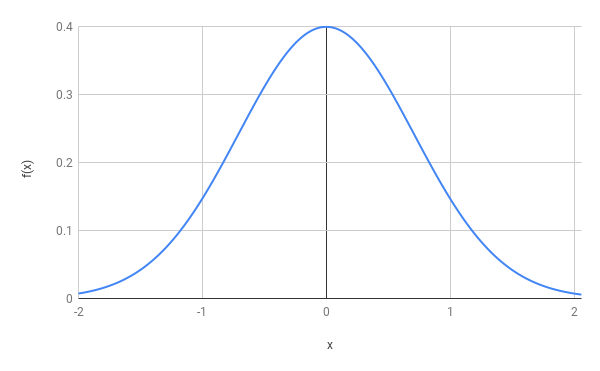
\includegraphics[width=1\linewidth]{figures/bell-shaped} 

}

\caption{\textsc{Bell Shaped Curve}.}\label{fig:bell-shaped}
\end{figure}

\subsection{Pareto Distributions}\label{pareto}

A key feature of the Pareto distribution is that the density
distribution does not go as fast to \(0\) as with the Gaussian
Distribution, as \(x\) becomes large.

In the context For concreteness, if \(x\) is population, then this would
mean that there are relatively many cities with a large size, especially
when assessed against the average city size, as well as its standard
deviation. Similarly, there are relatively many incomes that are much
larger than the mean. The Pareto Distribution is in fact defined by:
\[f(x)=a\frac{x_m^a}{x^{a+1}}.\]

For the cumulative distribution function, this implies:
\[1-F(x)=\left(\frac{x_m}{x}\right)^a.\]

\section{Some Real-Life
Distributions}\label{some-real-life-distributions}

\subsection{Natural Sciences}\label{natural-sciences}

Many distributions in the natural sciences are well described by a
Bell-shaped curve. In order to illustrate this, let us use the
\href{https://www.nlsinfo.org/}{National Longitudinal Surveys (NLS)}
from the Bureau of Labor Statistics which tracks the income, education,
and life circumstances of a large cohort of Americans across several
decades. The below figures shows the distribution of height in the
population, first for both genders, and then for male and female
separately.




\begin{figure}

{\centering 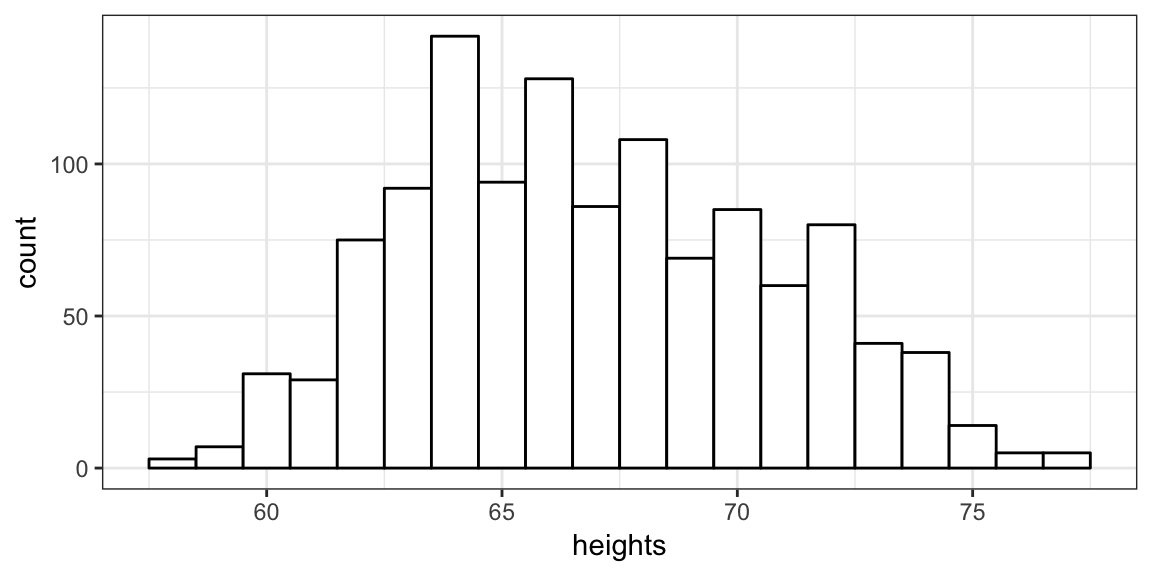
\includegraphics[width=1\linewidth]{ucla-19-fall2018_files/figure-latex/heights-fig-1} 

}

\caption{\textsc{Distribution of Height in the National
Longitudinal Surveys (NLS)}.}\label{fig:heights-fig}
\end{figure}




\begin{figure}

{\centering 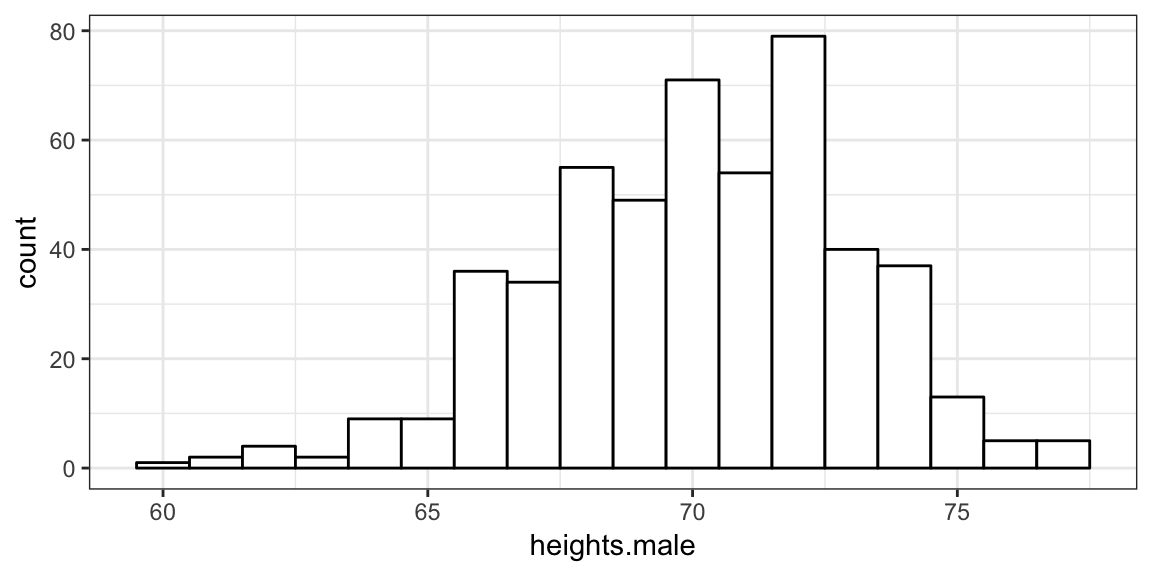
\includegraphics[width=1\linewidth]{ucla-19-fall2018_files/figure-latex/male-heights-fig-1} 

}

\caption{\textsc{Male Distribution of Height in the
National Longitudinal Surveys (NLS)}.}\label{fig:male-heights-fig}
\end{figure}




\begin{figure}

{\centering 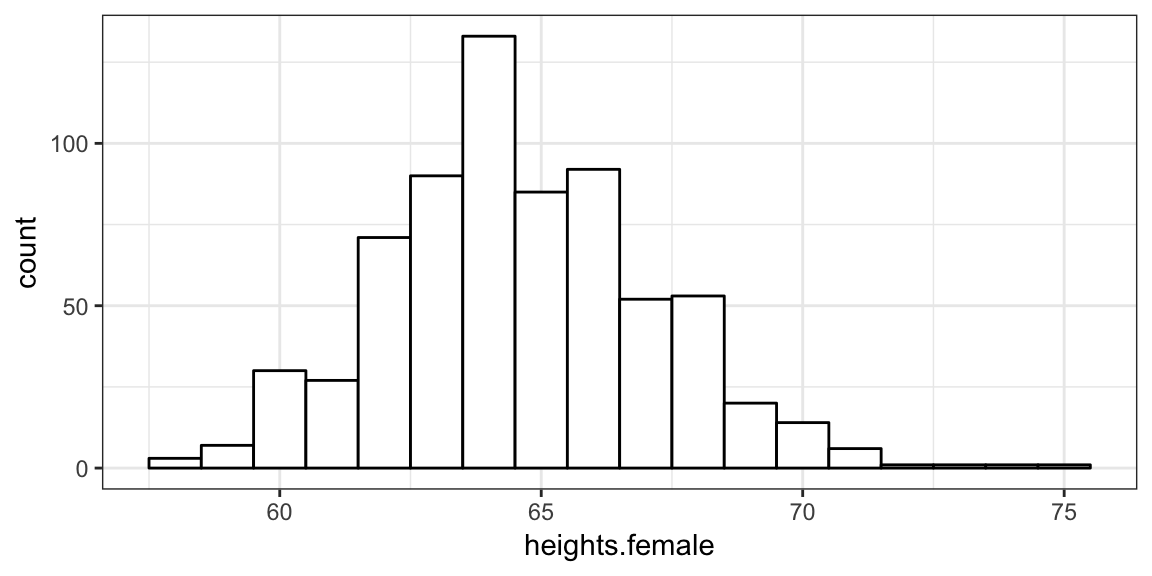
\includegraphics[width=1\linewidth]{ucla-19-fall2018_files/figure-latex/female-heights-fig-1} 

}

\caption{\textsc{Female Distribution of Height in the
National Longitudinal Surveys (NLS)}.}\label{fig:female-heights-fig}
\end{figure}

\subsection{Cities}\label{cities}

During the class, w have used
\href{https://docs.google.com/spreadsheets/d/1PJ9AjF0kDo-Fe5h3f4eAWZgccIjtn6urpA0Uk4OneXc/edit?usp=sharing}{this
Google Spreadsheet} in order to plot the city size distribution of
cities. We note that the result is something that is close to a linear
relationship, when the log rank is plotted against the log size, which
shows that the distribution is close to Pareto.



\begin{figure}

{\centering 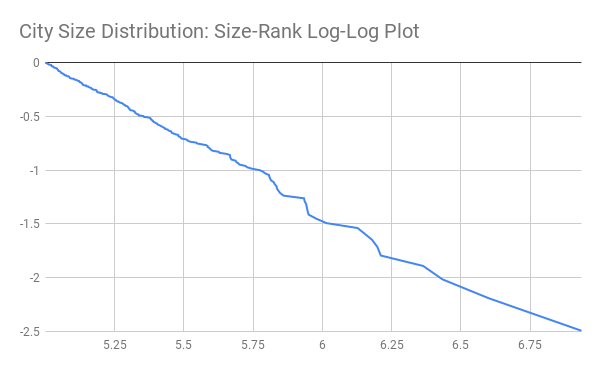
\includegraphics[width=1\linewidth]{figures/city-size-wikipedia} 

}

\caption{\textsc{City Size Distribution, Pareto Plot}.}\label{fig:city-size-wikipedia}
\end{figure}

We can also download everything in R directly. The data comes from the
following Wikipedia entry:
\href{https://en.wikipedia.org/wiki/List_of_United_States_cities_by_population}{List
of United States cities by population}.

Biggest cities:









\label{tab:unnamed-chunk-7}\textsc{Biggest Cities in the United States.}

rank

City

state

pop

1

New York{[}6{]}

New York

8,622,698

2

Los Angeles

California

3,999,759

3

Chicago

Illinois

2,716,450

4

Houston{[}7{]}

Texas

2,312,717

5

Phoenix

Arizona

1,626,078

6

Philadelphia{[}8{]}

Pennsylvania

1,580,863

7

San Antonio

Texas

1,511,946

8

San Diego

California

1,419,516

9

Dallas

Texas

1,341,075

10

San Jose

California

1,035,317

11

Austin

Texas

950,715

12

Jacksonville{[}9{]}

Florida

892,062

13

San Francisco{[}10{]}

California

884,363

14

Columbus

Ohio

879,170

15

Fort Worth

Texas

874,168

16

Indianapolis{[}11{]}

Indiana

863,002

17

Charlotte

North Carolina

859,035

18

Seattle

Washington

724,745

19

Denver{[}12{]}

Colorado

704,621

20

Washington{[}13{]}

District of Columbia

693,972

21

Boston

Massachusetts

685,094

22

El Paso

Texas

683,577

23

Detroit

Michigan

673,104

24

Nashville{[}14{]}

Tennessee

667,560

25

Memphis

Tennessee

652,236

26

Portland

Oregon

647,805

27

Oklahoma City

Oklahoma

643,648

28

Las Vegas

Nevada

641,676

\begin{figure}

{\centering 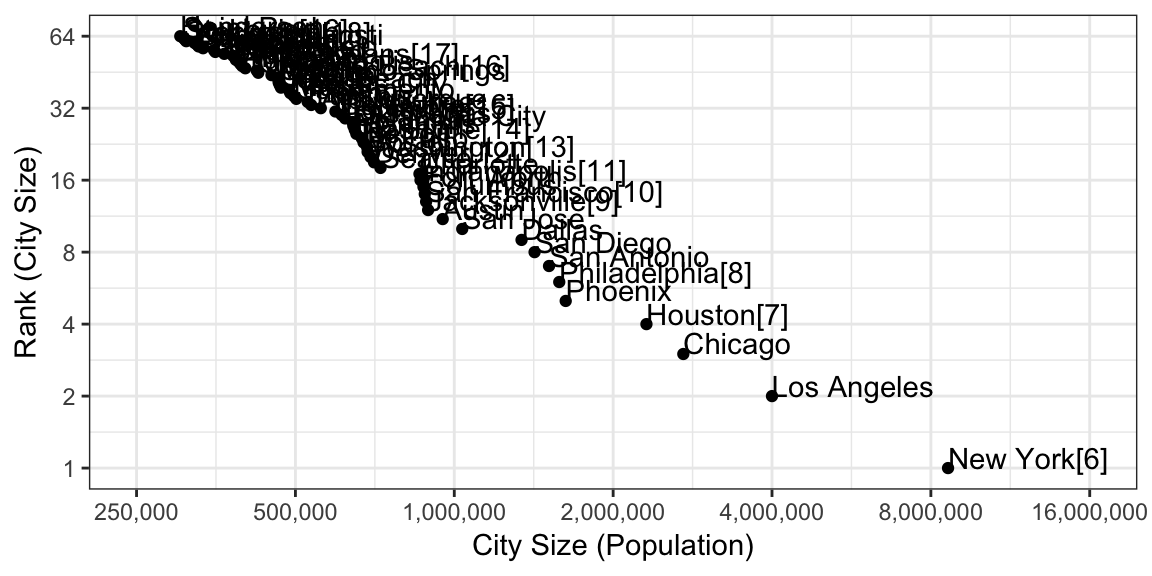
\includegraphics[width=1\linewidth]{ucla-19-fall2018_files/figure-latex/most-populated-US-cities-fig-1} 

}

\caption{\textsc{Most populated cities in the
U.S. (\textgreater{} 250,000), Pareto Plot.}}\label{fig:most-populated-US-cities-fig}
\end{figure}

\begin{figure}

{\centering 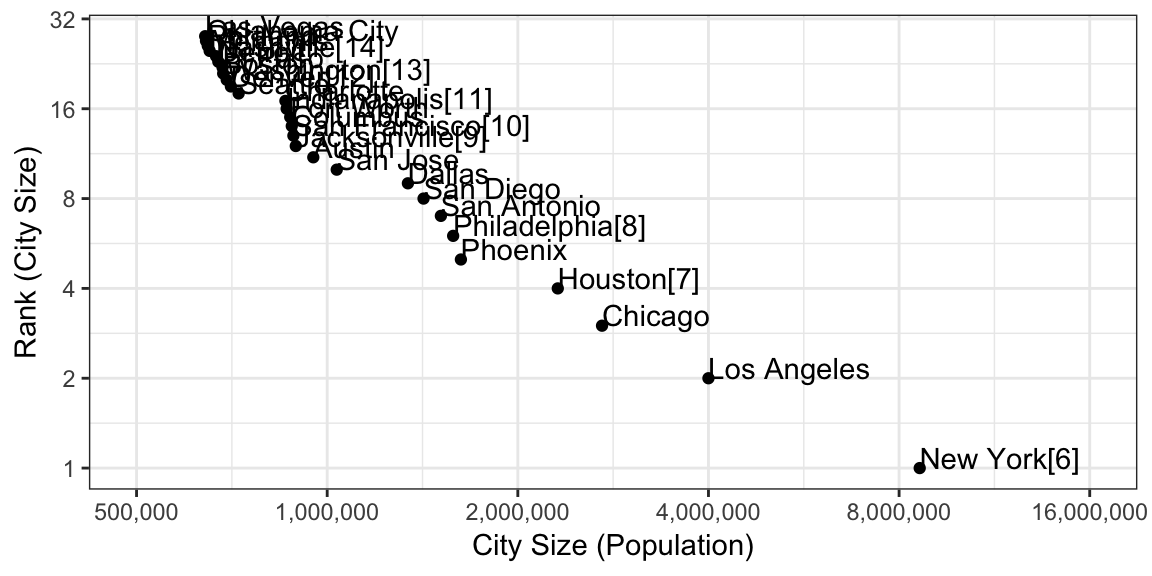
\includegraphics[width=1\linewidth]{ucla-19-fall2018_files/figure-latex/most-populated-US-cities-fig2-1} 

}

\caption{\textsc{Most populated cities in the
U.S. (\textgreater{} 500,000), Pareto Plot.}}\label{fig:most-populated-US-cities-fig2}
\end{figure}

\subsection{MSAs}\label{msas}

Instead of cities, we can look at MSAs instead. The data comes from the
following Wikipedia entry:
\href{https://en.wikipedia.org/wiki/List_of_metropolitan_statistical_areas}{List
of metropolitan statistical areas}.










The list of the 28 largest Metropolitan Statistical Areas is as follows.

\label{tab:unnamed-chunk-9}\textsc{Biggest Metropolitan Statistical Areas (MSAs)
in the United States.}

Metropolitan~statistical~area

2010 Census

New York-Newark-Jersey City, NY-NJ-PA MSA

19,567,410

Los Angeles-Long Beach-Anaheim, CA MSA

12,828,837

Chicago-Naperville-Elgin, IL-IN-WI MSA

9,461,105

Dallas-Fort Worth-Arlington, TX MSA

6,426,214

Houston-The Woodlands-Sugar Land, TX MSA

5,920,416

Washington-Arlington-Alexandria, DC-VA-MD-WV MSA

5,636,232

Miami-Fort Lauderdale-West Palm Beach, FL MSA

5,564,635

Philadelphia-Camden-Wilmington, PA-NJ-DE-MD MSA

5,965,343

Atlanta-Sandy Springs-Roswell, GA MSA

5,286,728

Boston-Cambridge-Newton, MA-NH MSA

4,552,402

Phoenix-Mesa-Scottsdale, AZ MSA

4,192,887

San Francisco-Oakland-Hayward, CA MSA

4,335,391

Riverside-San Bernardino-Ontario, CA MSA

4,224,851

Detroit-Warren-Dearborn, MI MSA

4,296,250

Seattle-Tacoma-Bellevue, WA MSA

3,439,809

Minneapolis-St.~Paul-Bloomington, MN-WI MSA

3,348,859

San Diego-Carlsbad, CA MSA

3,095,313

Tampa-St.~Petersburg-Clearwater, FL MSA

2,783,243

Denver-Aurora-Lakewood, CO MSA

2,543,482

Baltimore-Columbia-Towson, MD MSA

2,710,489

St.~Louis, MO-IL MSA

2,787,701

Charlotte-Concord-Gastonia, NC-SC MSA

2,217,012

Orlando-Kissimmee-Sanford, FL MSA

2,134,411

San Antonio-New Braunfels, TX MSA

2,142,508

Portland-Vancouver-Hillsboro, OR-WA MSA

2,226,009

Pittsburgh, PA MSA

2,356,285

Sacramento--Roseville--Arden-Arcade, CA MSA

2,149,127

Las Vegas-Henderson-Paradise, NV MSA

1,951,269

\begin{figure}

{\centering 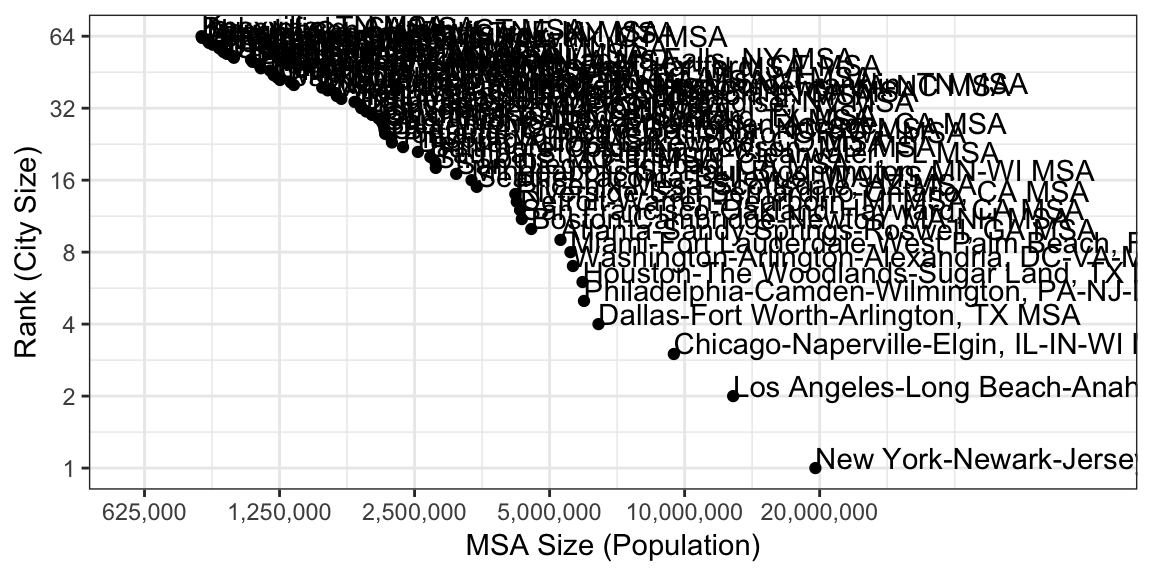
\includegraphics[width=1\linewidth]{ucla-19-fall2018_files/figure-latex/most-populated-US-MSAs-fig-1} 

}

\caption{\textsc{Most populated MSAs in the U.S.
(\textgreater{} 600,000), Pareto Plot.}}\label{fig:most-populated-US-MSAs-fig}
\end{figure}

\begin{figure}

{\centering 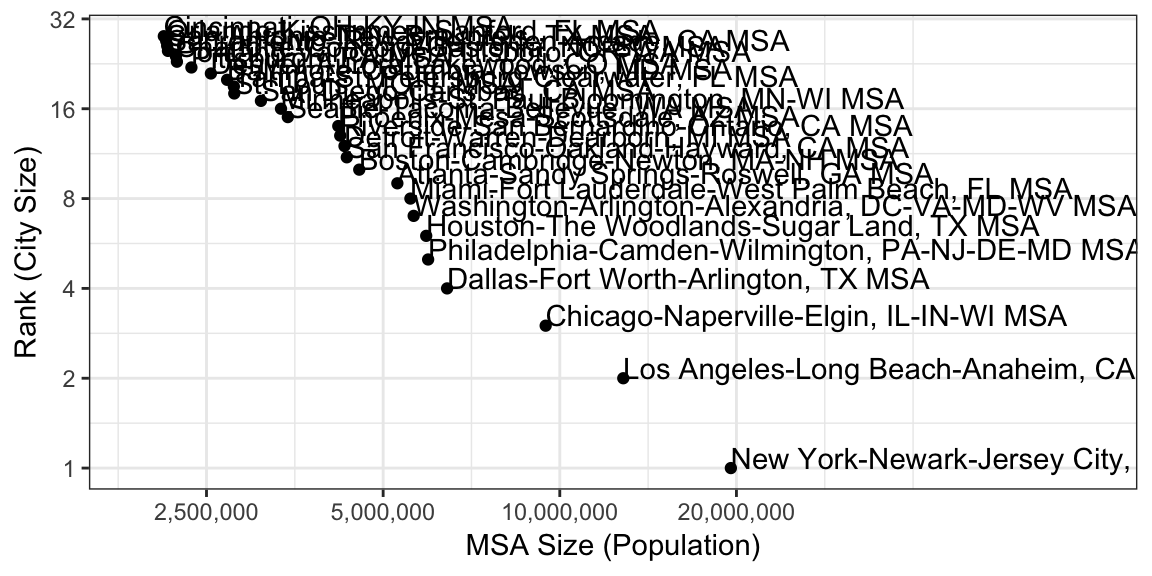
\includegraphics[width=1\linewidth]{ucla-19-fall2018_files/figure-latex/most-populated-US-MSAs-fig2-1} 

}

\caption{\textsc{Most populated MSAs in the
U.S. (\textgreater{} 1,900,000), Pareto Plot.}}\label{fig:most-populated-US-MSAs-fig2}
\end{figure}

\hypertarget{music-entertainment-superstars}{\chapter{Superstars in
Music, Sports and Entertainment}\label{music-entertainment-superstars}}

Sherwin Rosen, in the \emph{American Scholar}, writes:

\begin{quote}
Performers of first rank comprise a limited handful out of these small
totals and have very large incomes. There are also known to be
substantial differences in income between them and those in the second
rank, even though most consumers would have difficulty detecting more
than minor differences in a ``blind'' hearing.
\end{quote}

What Sherwin Rosen says is that there are very few differences in
talents at the very top.

\begin{quote}
The elusive quality of ``box office appeal,'' the ability to attract an
audience and generate a large volume of transactions, is the issue that
must be confronted. Recognition that one's personal market scale is
important, in the theory of income distribution has a long history, but
the idea has not been developed very extensively in the literature.
\end{quote}

\begin{quote}
Rest assured that prospective impresarios will receive no guidance here
on what makes for box office appeal, sometimes said to involve a
combination of talent and charisma in uncertain proportions. In the
formal model all that is taken for granted and represented by a single
factor rather than by two, an index q labeled talent or quality.
\end{quote}

\begin{quote}
Albert Rees is a good introduction to the size distribution of income.
The selectivity effects of differential talent and comparative advantage
on the skew in income distributions are spelled out in my 1978 article,
also see the references there. Melvin Reder's survey touches some of the
issues raised here.
\end{quote}

\begin{quote}
Of course social scientists and statisticians have had a long standing
fascination with rank-size relationships, as perusal of the many entries
in the Encyclopedia of the Social Sciences will attest.
\end{quote}

\section{Statistical Distributions for
Superstars}\label{statistical-distributions-for-superstars}

We use the methods we saw in \href{course2.html}{course 2} and plot the
log rank on the y axis against the log of the outcome of interest
(revenues, number of views, number of sales, etc.) We show that many of
these distributions associated to superstar phenomena display a
Pareto-like behavior in the tail: this means that there are very many
observations which deviate substantially from the mean, and that
earnings and success accrue disproportionately to the very top.

\subsection{Most-downloaded songs in the United
Kingdom}\label{most-downloaded-songs-in-the-united-kingdom}

The data comes from the following Wikipedia entry:
\href{https://en.wikipedia.org/wiki/List_of_most-downloaded_songs_in_the_United_Kingdom}{List
of most-downloaded songs in the United Kingdom}.




\label{tab:most-download-UK-songs}\textsc{List of most downloaded songs in
the United Kingdom.}

No.

Artist

Song

Copies sold{[}a{]}

1

Pharrell Williams

``Happy''

1,922,000{[}3{]}

2

Adele

``Someone Like You''

1,637,000+{[}4{]}

3

Robin Thicke featuring T.I. and Pharrell Williams

``Blurred Lines''

1,620,000+

4

Maroon 5 featuring Christina Aguilera

``Moves Like Jagger''

1,500,000+

5

Gotye featuring Kimbra

``Somebody That I Used to Know''

1,470,000+

6

Daft Punk featuring Pharrell Williams

``Get Lucky''

1,400,000+

7

The Black Eyed Peas

``I Gotta Feeling''

1,350,000+

8

Avicii

``Wake Me Up''

1,340,000+

9

Rihanna featuring Calvin Harris

``We Found Love''

1,337,000+

10

Kings of Leon

``Sex on Fire''

1,293,000+




\begin{figure}

{\centering 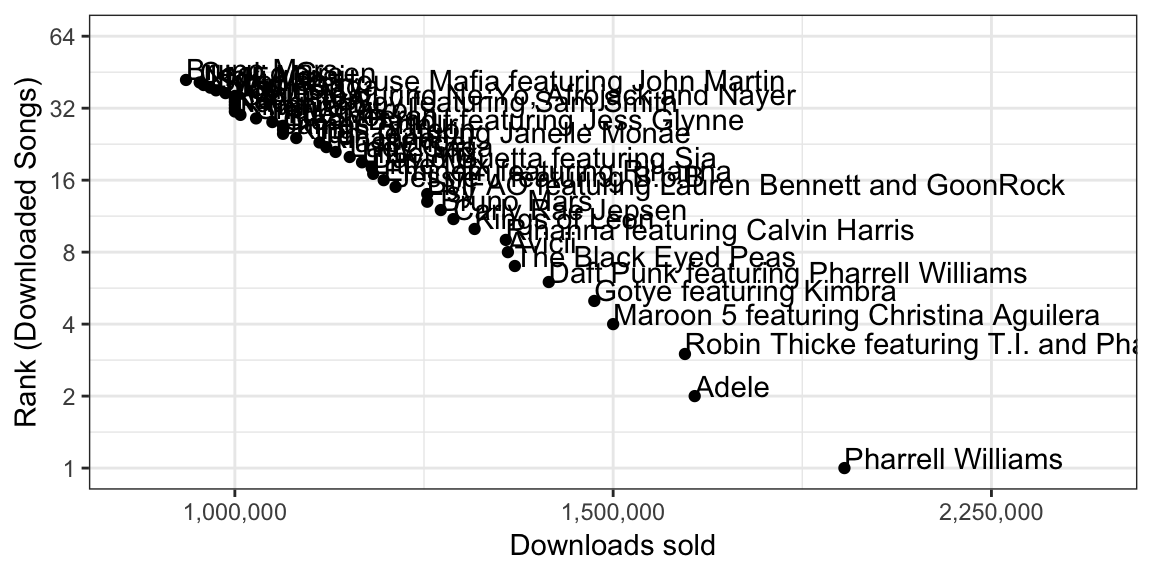
\includegraphics[width=1\linewidth]{ucla-19-fall2018_files/figure-latex/most-download-UK-songs-fig-1} 

}

\caption{\textsc{List of most downloaded songs
in the United Kingdom, Pareto Plot.}}\label{fig:most-download-UK-songs-fig}
\end{figure}

\subsection{Most-streamed songs on
Spotify}\label{most-streamed-songs-on-spotify}

The data comes from the following Wikipedia entry:
\href{https://en.wikipedia.org/wiki/List_of_most-streamed_songs_on_Spotify}{List
of most-streamed songs on Spotify}.



\label{tab:most-streamed-songs-spotify}\textsc{List of most streamed songs on Spotify.}

Rank

song

value

date

1

Shape of You

1981

6 January, 2017

2

One Dance

1592

5 April, 2016

3

Closer

1414

29 July, 2016

4

rockstar

1324

15 September, 2017

5

Thinking Out Loud

1212

21 June, 2014

6

Lean On

1180

2 March, 2015

7

Despacito (Remix)

1161

17 April, 2017

8

Love Yourself

1135

9 November, 2015

9

Sorry

1119

23 October, 2015

10

God's Plan

1104

19 January, 2018




\begin{figure}

{\centering 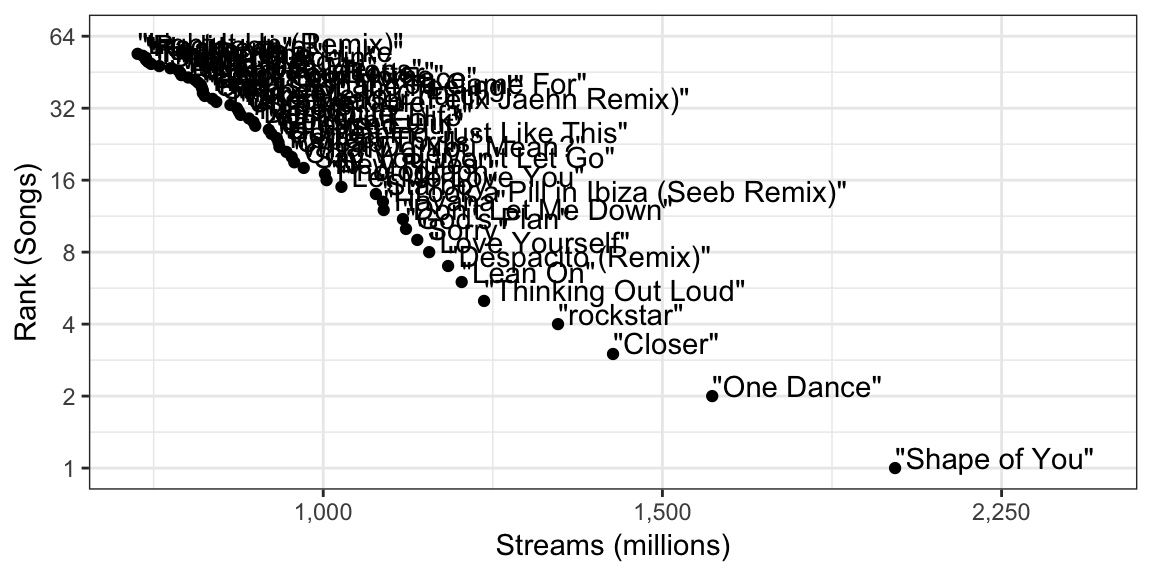
\includegraphics[width=1\linewidth]{ucla-19-fall2018_files/figure-latex/most-streamed-songs-spotify-fig-1} 

}

\caption{\textsc{List of most streamed
songs on Spotify, Pareto Plot.}}\label{fig:most-streamed-songs-spotify-fig}
\end{figure}

\subsection{Most-viewed YouTube
videos}\label{most-viewed-youtube-videos}

The data comes from the following Wikipedia entry:
\href{https://en.wikipedia.org/wiki/List_of_most-viewed_YouTube_videos}{List
of most-viewed YouTube videos}.



We then display the first rows of the data:

\label{tab:most-viewed-youtube}\textsc{List of most viewed YouTube videos.}

Rank

video

value

1

Despacito{[}16{]}

5.73

2

Shape of You{[}21{]}

3.91

3

See You Again{[}22{]}

3.88

4

Uptown Funk{[}29{]}

3.35

5

Masha and the Bear: Recipe for Disaster{[}30{]}

3.32

6

Gangnam Style{[}31{]}

3.24

7

Sorry{[}36{]}

3.04

8

Sugar{[}37{]}

2.82

9

Shake It Off{[}38{]}

2.68

10

Roar{[}39{]}

2.67

The
\href{https://www.youtube.com/watch?v=kJQP7kiw5Fk\&list=PLirAqAtl_h2r5g8xGajEwdXd3x1sZh8hC}{first
100 top Youtube videos} have been seen a couple \textbf{billion}
times:\\
-
\href{https://www.youtube.com/watch?v=kJQP7kiw5Fk\&list=PLirAqAtl_h2r5g8xGajEwdXd3x1sZh8hC}{Luis
Fonsi - Despacito ft. Daddy Yankee}: 5.7 Billion\\
-
\href{https://www.youtube.com/watch?v=JGwWNGJdvx8\&list=PLirAqAtl_h2r5g8xGajEwdXd3x1sZh8hC\&index=2}{Ed
Sheeran - Shape of You}: 3.88 Billion\\
-
\href{https://www.youtube.com/watch?v=RgKAFK5djSk\&list=PLirAqAtl_h2r5g8xGajEwdXd3x1sZh8hC\&index=3}{Wiz
Khalifa - See You Again ft. Charlie Puth}: 3.84 Billion\\
- etc.




\begin{figure}

{\centering 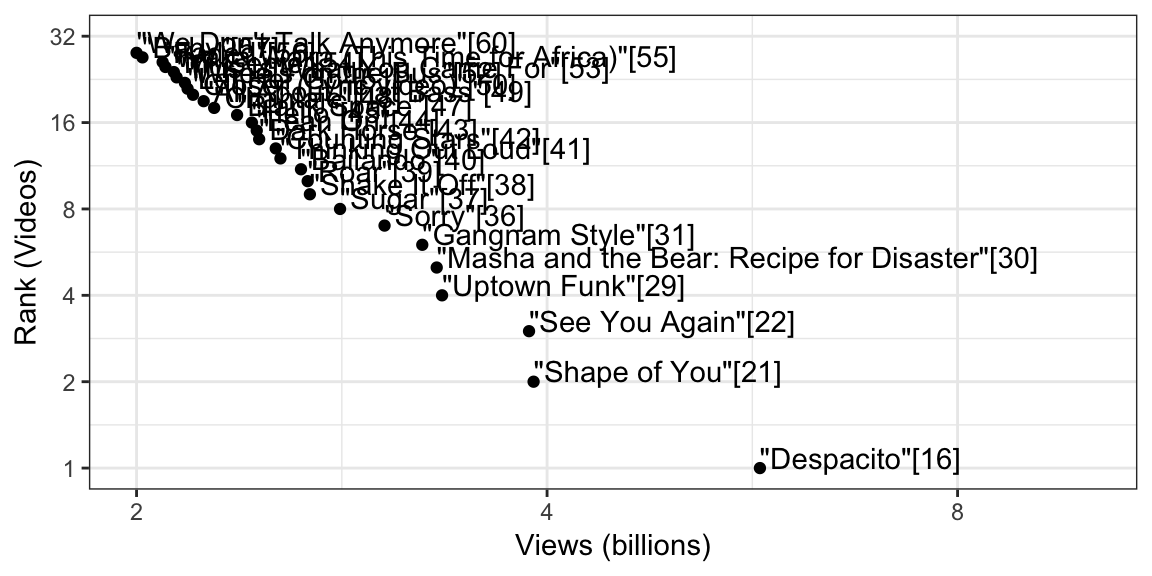
\includegraphics[width=1\linewidth]{ucla-19-fall2018_files/figure-latex/most-viewed-youtube-fig-1} 

}

\caption{\textsc{List of most viewed Youtube
videos, Pareto Plot.}}\label{fig:most-viewed-youtube-fig}
\end{figure}

\subsection{Highest paid American television
stars}\label{highest-paid-american-television-stars}

The data comes from the following Wikipedia entry:
\href{https://en.wikipedia.org/wiki/List_of_highest_paid_American_television_stars}{List
of highest paid American television stars}.

Network primetime salaries per episode




We then display the first rows of the data:

\label{tab:highest-paid-US-tv-stars}\textsc{Highest paid American Television
Stars.}

Name

Program

Role

Salary

Peter Dinklage

Game of Thrones

Tyrion Lannister

£2,000,000{[}a{]}

Nikolaj Coster-Waldau

Game of Thrones

Jaime Lannister

£2,000,000{[}a{]}

Lena Headey

Game of Thrones

Cersei Lannister

£2,000,000{[}a{]}

Emilia Clarke

Game of Thrones

Daenerys Targaryen

£2,000,000{[}a{]}

Kit Harington

Game of Thrones

Jon Snow

£2,000,000{[}a{]}

Charlie Sheen

Two and a Half Men

Charlie Harper

\$1.8 million

Ray Romano

Everybody Loves Raymond

Raymond Barone

\$1.7 million

Kelsey Grammer

Frasier

Frasier Crane

\$1.6 million

Tim Allen

Home Improvement

Tim Taylor

\$1.25 million

James Gandolfini

The Sopranos

Tony Soprano

\$1 million

\subsection{Highest grossing concert
tours}\label{highest-grossing-concert-tours}

The data comes from the following Wikipedia entry:
\href{https://en.wikipedia.org/wiki/List_of_highest-grossing_concert_tours}{List
of highest-grossing concert tours}. We first input the data from the
Wikipedia page, using the \texttt{rvest} package to extract tables from
the html source code:




We then display the first rows of the data:

\label{tab:highest-grossing-concert}\textsc{List of Highest Grossing Concert
Tours.}

Rank

Actual gross

Gross Infl Adj

Artist

1

\$736,421,584

\$801,130,818

U2

2

\$558,255,524

\$658,868,741

The Rolling Stones

3

\$523,033,675

\$533,331,898

Coldplay

4

\$480,900,000

\$490,368,636

Guns N' Roses

5

\$458,673,798

\$481,869,587

Roger Waters

6

\$441,121,000

\$495,041,025

AC/DC

7

\$408,000,000

\$465,399,721

Madonna

8

\$389,047,636

\$472,277,371

U2

9

\$364,300,000

\$364,300,000

Garth Brooks and Trisha Yearwood

10

\$362,000,000

\$411,460,278

The Police




\begin{figure}

{\centering 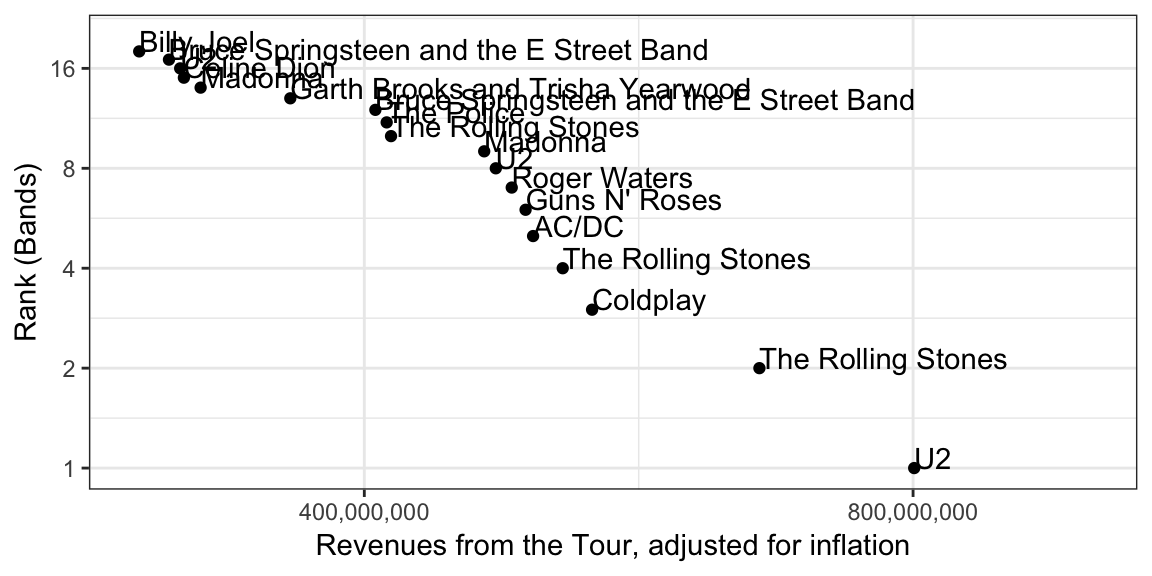
\includegraphics[width=1\linewidth]{ucla-19-fall2018_files/figure-latex/highest-grossing-concerts-fig-1} 

}

\caption{\textsc{List of Highest Grossing
Concerts, Pareto Plot.}}\label{fig:highest-grossing-concerts-fig}
\end{figure}

\subsection{Highest paid film actors}\label{highest-paid-film-actors}

The data comes from the following Wikipedia entry:
\href{https://en.wikipedia.org/wiki/List_of_highest_paid_film_actors}{List
of highest paid film actors}. We first input the data from the Wikipedia
page, using the \texttt{rvest} package to extract tables from the html
source code:




We then display the first rows of the data:

\label{tab:unnamed-chunk-11}\textsc{List of Highest Paid Film
Actors.}

Actor

Film

Year

Salary

Total income

Keanu Reeves

The Matrix ReloadedThe Matrix Revolutions

2003

\$30,000,000

\$156,000,000

Bruce Willis

The Sixth Sense

1999

\$14,000,000

\$100,000,000

Tom Cruise

Mission: Impossible 2

2000

\$100,000,000

Tom Cruise

War of the Worlds

2005

\$100,000,000

Will Smith

Men in Black 3

2012

\$100,000,000

Robert Downey, Jr.

Iron Man 3

2013

\$75,000,000

Sandra Bullock

Gravity

2013

\$20,000,000

\$70,000,000+

Tom Hanks

Forrest Gump

1994

\$70,000,000

Tom Cruise

Mission: Impossible

1996

\$70,000,000

Harrison Ford

Indiana Jones and the Kingdom of the Crystal Skull

2008

\$65,000,000

Jack Nicholson

Batman

1989

\$6,000,000

\$60,000,000

Leonardo DiCaprio

Inception

2010

\$59,000,000

Robert Downey, Jr.

Captain America: Civil War

2014

\$40,000,000

\$40,000,000+

Robert Downey, Jr.

Avengers: Age of Ultron

2014

\$40,000,000

Johnny Depp

Pirates of the Caribbean: On Stranger Tides

2011

\$35,000,000

\$55,000,000

\subsection{Largest sports contracts}\label{largest-sports-contracts}

The data comes from the following Wikipedia entry:
\href{https://en.wikipedia.org/wiki/List_of_largest_sports_contracts}{List
of largest sports contracts}.



We then display the first rows of the data:

\label{tab:unnamed-chunk-13}\textsc{Largest Sports Contracts.}

Player

Sport

length

value

Canelo Álvarez

Boxing

5 years (2018--2023)

\$365,000,000

Giancarlo Stanton

Baseball

13 years (2014--2027)

\$325,000,000

Alex Rodriguez1R

Baseball

10 years (2008--2017)

\$275,000,000

Alex Rodriguez2R

Baseball

10 years (2001--2010)

\$252,000,000

Miguel Cabrera

Baseball

8 years (2016--2023)

\$247,000,000

Robinson Cano

Baseball

10 years (2014--2023)

\$240,000,000

Albert Pujols

Baseball

10 years (2012--2021)

\$240,000,000

James Harden

Basketball

6 years (2017--2023)

\$228,000,000

Joey Votto

Baseball

10 years (2014--2024)

\$225,000,000

David Price

Baseball

7 years (2016--2022)

\$217,000,000

\section{Other examples}\label{other-examples}

\subsection{Billionaires from Forbes}\label{billionaires-from-forbes}

Preparing the data from the Forbes Website.



The first 25 billionaires are:

\label{tab:unnamed-chunk-15}\textsc{First 25 Billionaires.}

Rank

Billionaire

wealth

source

1

Bill Gates

79.2

Microsoft

2

Carlos Slim Helu \& family

77.1

telecom

3

Warren Buffett

72.7

Berkshire Hathaway

4

Amancio Ortega

64.5

Zara

5

Larry Ellison

54.3

Oracle

6

Charles Koch

42.9

diversified

6

David Koch

42.9

diversified

8

Christy Walton \& family

41.7

Wal-Mart

9

Jim Walton

40.6

Wal-Mart

10

Liliane Bettencourt \& family

40.1

L'Oreal

11

Alice Walton

39.4

Wal-Mart

12

S Robson Walton

39.1

Wal-Mart

13

Bernard Arnault \& family

37.2

LVMH

14

Michael Bloomberg

35.5

Bloomberg LP

15

Jeff Bezos

34.8

Amazon.com

16

Mark Zuckerberg

33.4

Facebook

17

Li Ka-shing

33.3

diversified

18

Sheldon Adelson

31.4

casinos

19

Larry Page

29.7

Google

20

Sergey Brin

29.2

Google

21

Georg Schaeffler

26.9

ball bearings

22

Forrest Mars Jr

26.6

candy

22

Jacqueline Mars

26.6

candy

22

John Mars

26.6

candy

25

David Thomson \& family

25.5

media




\begin{figure}

{\centering 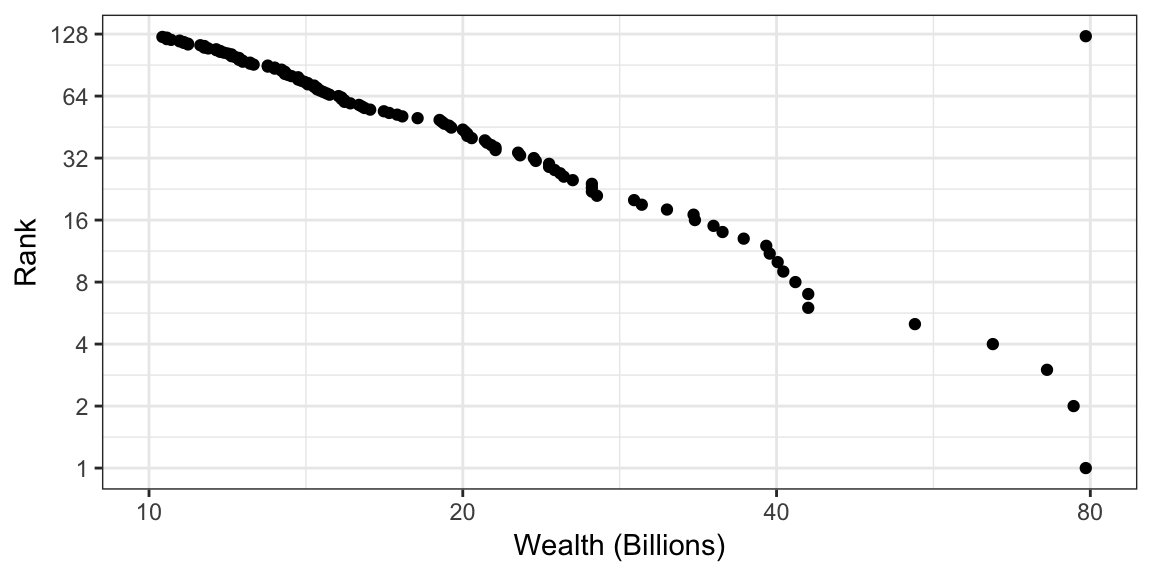
\includegraphics[width=1\linewidth]{ucla-19-fall2018_files/figure-latex/forbes-top-wealth-fig-1} 

}

\caption{\textsc{List of Top Wealth Holders according
to Forbes, Pareto Plot.}}\label{fig:forbes-top-wealth-fig}
\end{figure}

The Pareto distribution does not work very well for the very top (Bill
Gates is not rich enough!)




\begin{figure}

{\centering 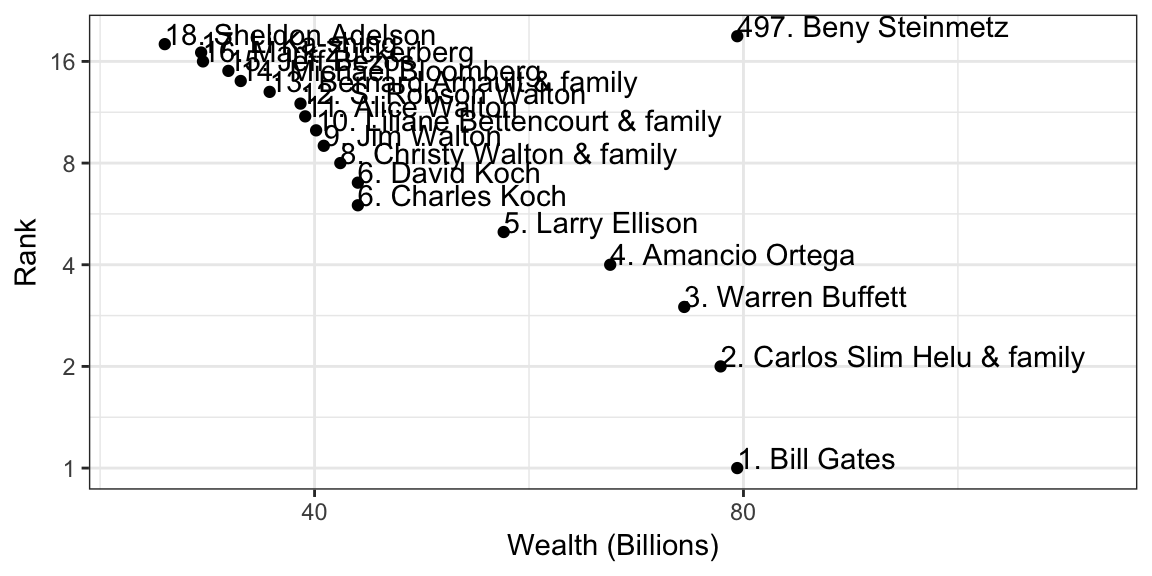
\includegraphics[width=1\linewidth]{ucla-19-fall2018_files/figure-latex/forbes-top-wealth-fig2-1} 

}

\caption{\textsc{List of Top Wealth Holders
according to Forbes (\textgreater{} 30 billion), Pareto Plot.}}\label{fig:forbes-top-wealth-fig2}
\end{figure}

\subsection{Salaries at the University of California
(UC)}\label{salaries-at-the-university-of-california-uc}

The salaries at the University of California are public and available at
this website: \url{https://ucannualwage.ucop.edu/wage/}

The distribution in the tail at the University of California is really
well approximated by a Pareto distribution. Below is the plot of wages
higher than \$250K.




\begin{figure}

{\centering 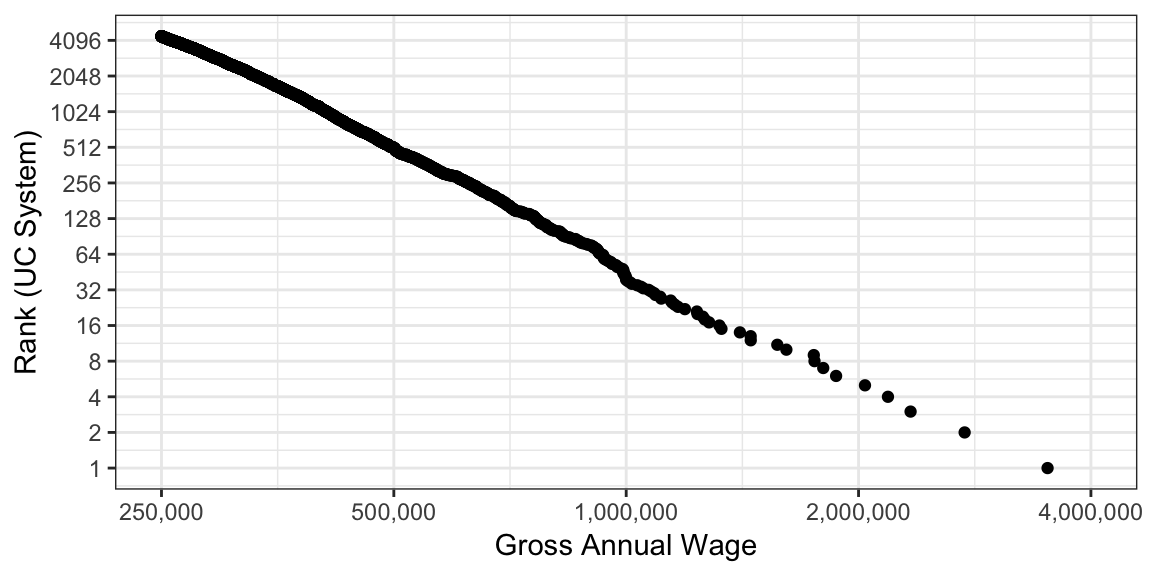
\includegraphics[width=1\linewidth]{ucla-19-fall2018_files/figure-latex/uc-system-wage-distribution-1} 

}

\caption{\textsc{Distribution of Wage Incomes
in the UC System (\textgreater{}250 K), Pareto Plot.}}\label{fig:uc-system-wage-distribution}
\end{figure}

The distribution in the tail at the University of California is really
well approximated by a Pareto distribution. Below is the plot of wages
higher than \$400K.




\begin{figure}

{\centering 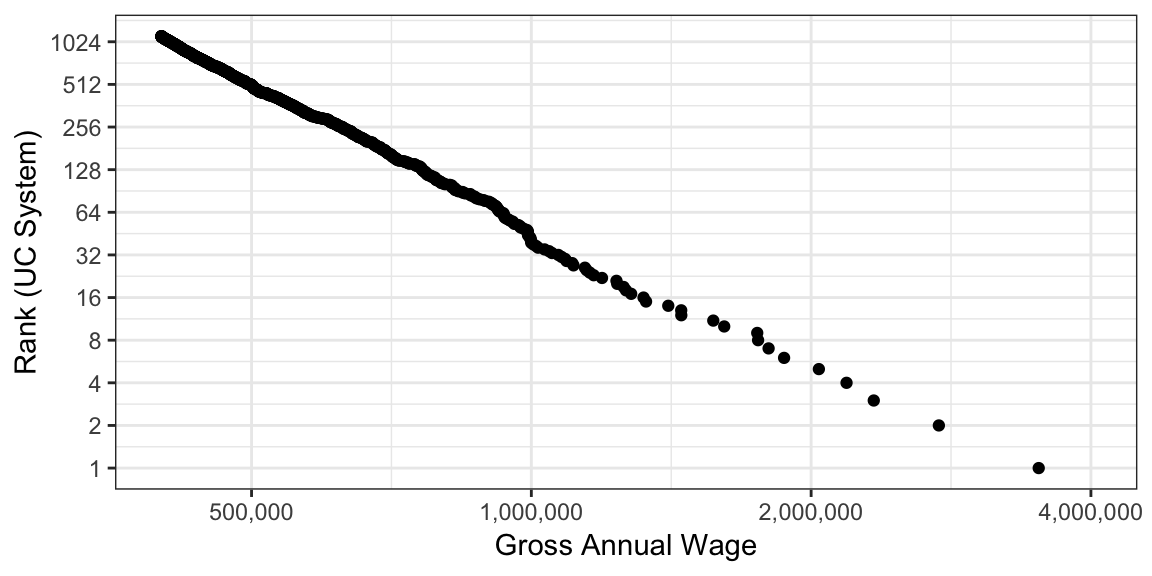
\includegraphics[width=1\linewidth]{ucla-19-fall2018_files/figure-latex/uc-system-wage-distribution-400K-1} 

}

\caption{\textsc{Distribution of Wage
Incomes in the UC System (\textgreater{}400 K), Pareto Plot.}}\label{fig:uc-system-wage-distribution-400K}
\end{figure}

Below is a zoom on the distribution of wages higher than 1.5 million
annual. You can see that the highest paid superstars on campus are the
Head Coaches, and superstar physicians. Again, it is striking that these
distributions are very well approximated by a Pareto distribution.




\begin{figure}

{\centering 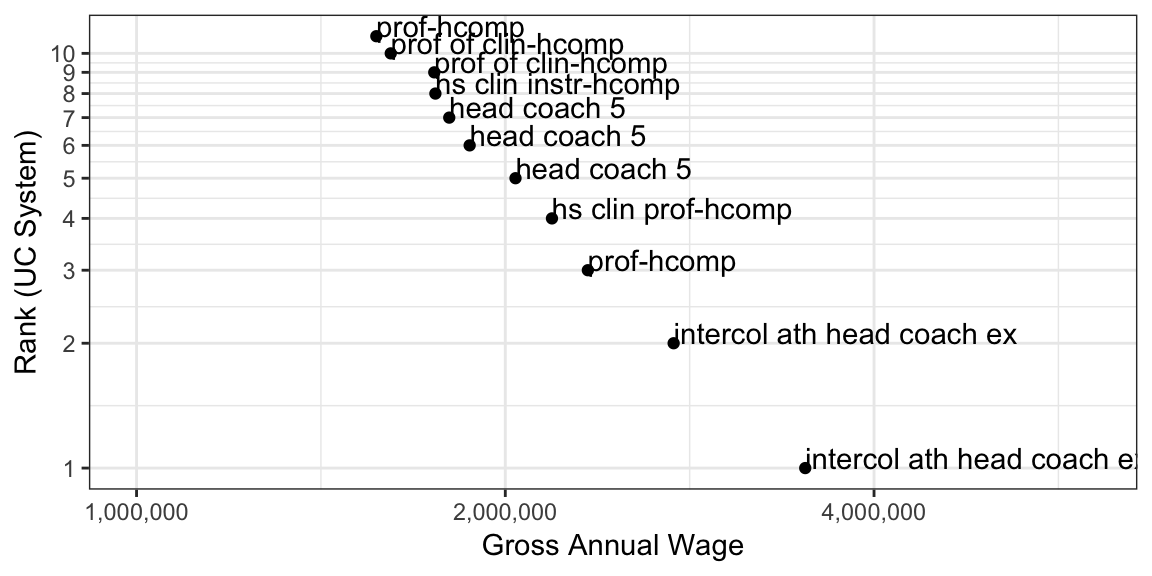
\includegraphics[width=1\linewidth]{ucla-19-fall2018_files/figure-latex/uc-system-wage-distribution-1-5million-1} 

}

\caption{\textsc{Distribution of
Wage Incomes in the UC System (\textgreater{}400 K), Pareto Plot.}}\label{fig:uc-system-wage-distribution-1-5million}
\end{figure}

\subsection{Market for Executive Officers in large
firms}\label{market-for-executive-officers-in-large-firms}

Again, from Sherwin Rosen:

\begin{quote}
Such considerations are important for understanding the market for
executive officers in large firms. Unusually good information on
executive compensation is available from public proxy statements
circulated to stockholders by requirement of the Securities and Exchange
Commission. Examination of these statements is instructive. They reveal
Superstar-scale rewards that are highly concentrated among the top
half-dozen executives in these firms. More detailed study indicates that
the top incomes vary systematically with the size of the organization.
Large firms pay executives more than smaller firms do. Even the
occasional, well-publicized dollar-a-year man falls in line once stock
options, pensions, and other forms of deferred compensation are properly
accounted. The value to the organization of good top-level decisions and
avoidance of bad decisions is abundantly clear once the nature of
control of resources on such a vast scale is considered.
\end{quote}

\begin{quote}
Common use of the term Officer for corporate executives Suggests certain
parallels with the military. A good or bad decision by a platoon leader
does not have much effect on the overall fortunes of war, but the same
cannot be said of decisions made by the chief strategists. The value of
extra talent is much larger at the top of the organizational hierarchy
than at the bottom because those decisions percolate through the
enterprise, and they have much further to travel in a larger enterprise
than in a smaller one.
\end{quote}

\hypertarget{presentations1}{\chapter{Presentations
1}\label{presentations1}}

\begin{enumerate}
\def\labelenumi{\arabic{enumi}.}
\item
  \href{https://doi.org/10.1257/jep.27.3.3}{Alvaredo, Facundo, Anthony
  B. Atkinson, Thomas Piketty, and Emmanuel Saez. ``The Top 1 Percent in
  International and Historical Perspective.'' Journal of Economic
  Perspectives 27, no. 3 (September 2013): 3--20.}\\
  \textbf{2:00-2:25PM: Stephanie Foo - Evan Veatch}
\item
  \href{https://doi.org/10.1257/jep.27.3.35}{Kaplan, Steven N., and
  Joshua Rauh. ``It's the Market: The Broad-Based Rise in the Return to
  Top Talent.'' Journal of Economic Perspectives 27, no. 3 (September
  2013): 35--56.}\\
  \textbf{2:25-2:50PM: Jessica Wong - Mingrui (Tony) Ma}
\item
  \href{https://doi.org/10.1257/jep.27.3.57}{Bivens, Josh, and Lawrence
  Mishel. ``The Pay of Corporate Executives and Financial Professionals
  as Evidence of Rents in Top 1 Percent Incomes.'' Journal of Economic
  Perspectives 27, no. 3 (September 2013): 57--78.}\\
  \textbf{3:00-3:25PM: Maxwell Grollman - Kai Colorado}
\item
  \href{https://doi.org/10.1257/jep.27.3.21}{Mankiw, N. Gregory.
  ``Defending the One Percent.'' Journal of Economic Perspectives 27,
  no. 3 (September 2013): 21--34.}\\
  \textbf{3:25-3:50PM: Bella Eagan - Kavvya Gupta}
\end{enumerate}

\hypertarget{presentations2}{\chapter{Presentations
2}\label{presentations2}}

\begin{enumerate}
\def\labelenumi{\arabic{enumi}.}
\setcounter{enumi}{4}
\item
  \href{https://doi.org/10.1257/jep.26.2.119}{Haskel, Jonathan, Robert
  Z. Lawrence, Edward E. Leamer, and Matthew J. Slaughter.
  ``Globalization and U.S. Wages: Modifying Classic Theory to Explain
  Recent Facts.'' Journal of Economic Perspectives 26, no. 2 (May 2012):
  119--40.}\\
  \textbf{2:00-2:25PM: Sana Lalani - Nadeen Malik}
\item
  \href{https://doi.org/10.1257/jep.27.3.79}{Corak, Miles. ``Income
  Inequality, Equality of Opportunity, and Intergenerational Mobility.''
  Journal of Economic Perspectives 27, no. 3 (September 2013):
  79--102.}\\
  \textbf{2:25-2:50PM: Adriana Conte - Stephanie Ciceri}
\item
  \href{https://doi.org/10.1257/jep.27.3.103}{Bonica, Adam, Nolan
  McCarty, Keith T. Poole, and Howard Rosenthal. ``Why Hasn't Democracy
  Slowed Rising Inequality?'' Journal of Economic Perspectives 27, no. 3
  (September 2013): 103--24.}\\
  \textbf{3:00-3:25PM: Ethan Chong - Emilia Davies}
\end{enumerate}

\chapter{Conclusion}\label{concluding-superstars}

\section{Importance of hard work}\label{importance-of-hard-work}

\section{Importance of luck}\label{importance-of-luck}

Ed Sheeran: social media -- being likeable.

No one has to buy your record anymore. People buy your record if you are
likeable.

Anyone who comes across as a dick does not seel any records

Playing in large venues

Go out and touring

96\%: revenues comes from Live

Wembley: 80,000 people Size of stadiums

I don't a bit luxury yacht and a private jet. What i want to do is live
in a country zzon and eat fish and chips.

I think you have to work for talent. I tghink persistence is worth more
than talent

\begin{verbatim}
# [1] "Sorry I don't know how to embed videos in PDF"
# [1] "Use the html version, or the link: https://youtu.be/O-Nh1QdpZPg?t=497"
\end{verbatim}

Music is so subjective that you don't have asmuch competitiion

it's not like they are stealing customers everyone's like in their own
lanes

perofrmance slots: in the grammy's in terms of existing as a musician

i have a competitive streak against mysef

that's not to take away from any other musician my competitive streak is
more with myself

Find your passion and you'll be ok.

Writing very quickly: Beatles, some songs that would not have made it
into the albums, are the ones that people like most nowadays.

i can't say who my

\section{rankings}\label{rankings}

Time 100:

\url{https://en.wikipedia.org/wiki/Time_100}

\section{Famous UCLA Graduates}\label{famous-ucla-graduates}

\begin{verbatim}
# [1] "Sorry I don't know how to embed videos in PDF"
# [1] "Use the html version, or the link: https://www.youtube.com/embed/1CLhqjOzoyE"
\end{verbatim}

\section{Advice from Ed Sheeran}\label{advice-from-ed-sheeran}

I just make the record for me.

You are a songwriter rather than a perofrmer

I never thought I would play a sadium: coldplay, U2, Bruce Springsteen I
will always be a songwriter.

\section{Charlie Rose Interviews}\label{charlie-rose-interviews}

\subsection{David Bowie}\label{david-bowie}

\url{https://www.youtube.com/watch?v=t8CNhakfB7c}

Inside Job: \url{https://www.youtube.com/watch?v=vS0hj4kiqsA}

300 million

Risk takers, compulsive

If you had looked you would have found things.

Because then you would have found the culprits

Frederic Mishkin

\bibliography{19.bib}


\end{document}
